% Select document class: 12 point, article
\documentclass[12pt]{article}

\usepackage{makecell}
\usepackage{inputenc}
%\def\includegraphic{}
%\def\includegraphics{}
\usepackage{graphicx}
%\usepackage{xr-hyper}
%\usepackage{xr}
%\usepackage{hyperref}
\usepackage{multirow}
\usepackage{colortbl}
%\usepackage{mathtools}
\usepackage{amsmath}

\def\code#1{\texttt{#1}}
\usepackage{soul}
\newcommand{\red}[1]{\textcolor{red}{#1}}
\newcommand{\blue}[1]{\textcolor{blue}{#1}}

\definecolor{salmon}{rgb}{1,0.4,0}

% AMS = American Mathematical Society; math, symbols, theorems, fonts
\usepackage{amsmath, amssymb, amsthm, amsfonts}

% Enhanced graphics support (https://ctan.org/pkg/graphicx?lang=en)
\usepackage{graphicx}

% Set default graphics path (replace 'figures/' with whatever directory your images are in)
%\graphicspath{{figures/}}
 
% Control layout of itemize, enumerate, description (https://ctan.org/pkg/enumitem?lang=en)
\usepackage{enumitem}

% Header and footer formatting options
\usepackage{fancyhdr}

% Control float placement. [section] = "stop floats at section boundaries is to change the definition of “\section” to include “\FloatBarrier”"
\usepackage[section]{placeins}

% Hypertext (links) in LaTeX. [option] = remove color and border on links.
\usepackage[hidelinks]{hyperref}

%\usepackage[all]{xy}
%\usepackage{mathtools}

% Programming facilities for LaTeX class and package authors
\usepackage{etoolbox}

% Indent first paragraph of every 'chapter' aka section
\usepackage{indentfirst}

% Title formatting option. [explicit] = make titles all caps
\usepackage[explicit]{titlesec}

% Standard package for selecting font encodings. [T1] = Support for accented characters
\usepackage[T1]{fontenc}

% Charter fonts
\usepackage{charter}

%\usepackage[expert]{mathdesign}

% Control table of contents, figures, etc
\usepackage{tocloft}

% Set space between lines. [option] = Double/single spacing necessary for properly formatting ToC/LoFT and titles.
\usepackage[doublespacing]{setspace}

% Create normal/logarithmic plots in two and three dimensions
\usepackage{pgfplots}
% Request a specific version
\pgfplotsset{compat=1.5}

\newcommand\scalemath[2]{\scalebox{#1}{\mbox{\ensuremath{\displaystyle #2}}}}

% Modify section headers (aka chapters) to be: centered, single space, large, bold, preceded with the word 'CHAPTER 'and with 0.4 em of space before title 
\titleformat{\section}[block]{\centering\singlespace\large\bf}{CHAPTER \thesection \hspace{0.4em} \MakeUppercase{#1}}{0em}{}{}

% Modify unnumbered section headers (aka chapters) to be: centered, single space, large, bold, preceded with the word 'CHAPTER 'and with 0.4 em of space before title 
%   We use unnumbered section headers for Acknowledgements, Dedication, Bio, etc. for consistency
\titleformat{name=\section,numberless}[block]{\centering\singlespace\large\bf}{\hspace{0.4em} \MakeUppercase{#1}}{0em}{}{}

% Remove spacing left of, above, and below sections and subsections
%\titlespacing{command}{left spacing}{before spacing}{after spacing}[right]
\titlespacing{\section}{0pt}{0pt}{0pt}
\titlespacing{\subsection}{0pt}{0pt}{0pt}
\titlespacing{\subsubsection}{0pt}{0pt}{0pt}

% Modify TOC entries with tocloft: insert the word 'Chapter ' and then add 6em of space after the word
\renewcommand{\cftsecleader}{\cftdotfill{\cftdotsep}}
\renewcommand{\cftsecpresnum}{Chapter }
\cftsetindents{section}{0em}{6em}

% Call the other parts of the document 'part' and make the table of contents print them correctly
\renewcommand{\cftpartfont}{}
\renewcommand{\cftpartpagefont}{}
\renewcommand{\cftpartleader}{\cftdotfill{\cftdotsep}}
\renewcommand{\cftbeforepartskip}{0em}
\renewcommand{\cftpartindent}{1.5em}

% Change spacing above chapters in toc, remembering that they are really sections
\setlength{\cftbeforesecskip}{0em}

% Adds space after ToC entries to make them appear double-spaced
\renewcommand\cftsecafterpnum{\vskip\baselineskip}
\renewcommand\cftsubsecafterpnum{\vskip\baselineskip}
\renewcommand\cftsubsubsecafterpnum{\vskip\baselineskip}
\renewcommand\cftpartafterpnum{\vskip\baselineskip}

% Add space after LoF entries to make them appear double-spaced
\renewcommand\cftfigafterpnum{\vskip\baselineskip}

% Add space after LoT entries to make them appear double-spaced
\renewcommand\cfttabafterpnum{\vskip\baselineskip}

% Remove extra space above and below theorems, lemmas, props, etc. The important point in the following is: 0pt preskip and 0pt postskip
\makeatletter
\def\thm@space@setup{\thm@preskip=0pt
\thm@postskip=0pt}
\makeatother
\newtheoremstyle{newstyle}      
{} % Aboveskip 
{} % Below skip
{\mdseries} % Body font e.g.\mdseries,\bfseries,\scshape,\itshape
{} % Indent
{\bfseries}  % Head font e.g.\bfseries,\scshape,\itshape
{.} % Punctuation afer theorem header
{ } % Space after theorem header
{} % Heading

% The above does not fix the spacing around proof environments; use the following to fix: The crucial point is "topsep0\p@", i.e., topsep = 0 pt. The rest is essentially copied from the standard AMS environment.
\makeatletter
\renewenvironment{proof}[1][\proofname]{\par
  \pushQED{\qed}%
  \normalfont \topsep0\p@\relax
  \trivlist
  \item[\hskip\labelsep\itshape
  #1\@addpunct{.}]\ignorespaces 
}{
  \popQED\endtrivlist\@endpefalse
}
\makeatother

% Remove default "References" text from \bibliography call
%   Removing this code will cause "References" to appear twice in the bibliography: once for the \thebibliography call and once for the \section*{References} call
\patchcmd{\thebibliography}{\section*{\refname}}{}{}{}

% Remove spacing between bibliography entries
% Set "OLDthebibliography" to be "thebibliography"
\let\OLDthebibliography\thebibliography
% Renew command with 0pt spacing for paragraph and item separation
\renewcommand\thebibliography[1]{
    \OLDthebibliography{#1}
    \setlength{\parskip}{0pt}
    \setlength{\itemsep}{0pt plus 0.3ex}
}

% Formatting
\usepackage[left=1in,right=1in, top=1in, bottom=1in]{geometry}
% \arraystretch = the FACTOR for spacing between two rows (Default = 1) 
\renewcommand{\arraystretch}{0.85}
% \baselinestretch = The spacing between lines in a document (used for "double spacing")
\renewcommand{\baselinestretch}{2}
% \headrulewidth = "The thickness of a line under the header and above the footer"
\renewcommand{\headrulewidth}{0pt}

% Define the StarTeX mathematical symbol
\newcommand{\Mdef}[2]{\newcommand{#1}{\relax \ifmmode #2 \else $#2$\fi}}

% Spacing commands, which may or may not be used in the following.
\newcommand{\one}{{\rm \bf1}\hspace*{-0.035in} {\rm l}}
\newcommand{\nd}{\noindent}
\def\para#1{\vskip 0.4\baselineskip\noindent{\bf #1}}
\newcommand{\Vspc}{\vspace*{0.1in}}

\newcommand{\ID}{\index}
\makeatletter \@addtoreset{equation}{section} \makeatother

% Section Labeling
\renewcommand{\thesection}{\arabic{section}}

% Equation Numbering Ex. Section 3, Equation 2 = Equation 3.2
\renewcommand{\theequation}{\thesection.\arabic{equation}}

\renewcommand{\cftsecfont}{}
\renewcommand{\cftsecpagefont}{}

% List of Tables edits
\renewcommand{\cfttabpresnum}{Table }
\renewcommand{\cfttabindent}{1.0em}
\renewcommand{\cfttabnumwidth}{5.0em}

% List of Figures edits
\renewcommand{\cftfigpresnum}{Figure }
\renewcommand{\cftfigindent}{1.0em}
\renewcommand{\cftfignumwidth}{5.5em}

% Start document
\begin{document}

% Compile the title and jump to new page
% Create title (centered and bold font)
\centerline{\uppercase{\bf Disease understanding and drug repurposing}}
\vspace{-0.4cm}
\centerline{\uppercase{\bf through pathway analysis}}
%\vspace{-0.4cm}
%\centerline{\bf TITLE LINE 3 (if needed)}

\vskip-0.4cm
\thispagestyle{empty}

% Center the following text:
\begin{center}
    \vspace{-0.4cm}
    by \\
    {\bf \uppercase{Tuan Minh Nguyen}}\\ % Full Name
    {\bf \uppercase{Dissertation}}\\  % THESIS (MS Thesis) or DISSERTATION (Ph.D Dissertation)
    Submitted to the Graduate School,\\
    of Wayne State University,\\
    Detroit, Michigan\\
    in partial fulfillment of the requirements\\
    for the degree of\\
    {\bf DOCTOR OF PHILOSOPHY} % MASTER OF SCIENCE / MASTER OF ARTS / DOCTOR OF EDUCATION / DOCTOR OF PHILOSOPHY / etc.
\end{center}

% Left-align the following text:
\begin{flushleft}
    \vspace*{-0.20in}
    \hspace*{3.09in}2025 % Use the year you will graduate
    \hspace*{3.09in}MAJOR: COMPUTER SCIENCE\\ % Major here
    \hspace*{3.09in}Approved By:\\
     \vspace{1cm}
     \hspace*{3.09in}---------------------------------------------------\\
    \vspace*{-0.25in}
    \hspace*{3.09in}Dr. Sorin Draghici\hspace*{1in} Date\hspace*{0.1in}\\
       \vspace{1cm}
    \vspace*{-0.25in}
         \hspace*{3.09in}---------------------------------------------------\\
            \vspace{1cm}
             \vspace*{-0.25in}
         \hspace*{3.09in}---------------------------------------------------\\
            \vspace{1cm}
             \vspace*{-0.25in}
         \hspace*{3.09in}---------------------------------------------------\\
         
    % Add these lines below for the cover that will be signed by advisors
    % WSU Graduate School asked that these lines below be removed for publiction
    %   Ex. When printing copies for dissertation committee, UNCOMMENT THE LINES BELOW.
    %   Ex. When sending a PDF of the thesis to WSU Grad school for format check (through ETD), COMMENT THE LINES BELOW. 
    %\bigskip
    %\hspace*{3.09in}-----------------------------------------------------------\\
    %\medskip
    %\hspace*{3.09in}-----------------------------------------------------------\\
    %\medskip
    %\hspace*{3.09in}-----------------------------------------------------------\\
    %\medskip
    %\hspace*{3.09in}-----------------------------------------------------------
\end{flushleft}

\newpage

% Begin roman numbering starting with page 2
%   WSU formatting requires: No pg number on title, pg numbering begins with page 2, pg numbering begins in roman numerals
\pagestyle{fancy} \chead{} \rhead{} \lhead{}
\pagenumbering{roman} \lfoot{}\cfoot{\thepage}\rfoot{}
\setcounter{page}{2}

% Compile dedication page
\phantomsection
% Use unnumbered section for dedication
\section*{DEDICATION}

% Add reference to the table of contents {toc} at the section level {section} titled "Dedication" {Dedication}
\addcontentsline{toc}{section}{Dedication}
\begin{center}
To my parents with their unlimited support, \\my wife for her dedication to the family,\\ and my son for his smile. \end{center}

\newpage

% Compile acknowledgements page
\phantomsection
% Use unnumbered section for acknowledgements
\section*{ACKNOWLEDGEMENTS}

% Add reference to the table of contents {toc} at the section level {section} titled "Acknowledgements" {Acknowledgements}
\addcontentsline{toc}{section}{Acknowledgements}

	I would like to express my deepest gratitude to my supervisor, Dr. Sorin Dr\u{a}ghici, for his invaluable guidance, continuous support, and encouragement throughout my research journey. His insightful feedback and unwavering patience has been instrumental in shaping this dissertation and my growth as a researcher.

I am also profoundly grateful to my parents for their unconditional love, support, and sacrifices that have made this journey possible. Their belief in me has been a constant source of motivation.

To my wife, Truc Bui, your patience, understanding, and unwavering support have been my greatest strength. Your encouragement has kept me going through the challenges of this journey, and for that, I am forever thankful.

I would also like to extend my appreciation to my current and former lab mates, especially Tin Nguyen, Adib Shafi, Douglas Craig, Cristina Mitrea and Radu Vanciu, whose collaboration, insightful discussions, and camaraderie have made this experience both enriching and enjoyable. Their support and shared knowledge have greatly contributed to this work.

Finally, I acknowledge everyone who has contributed, directly or indirectly, to the completion of this dissertation. Your support and encouragement have meant the world to me.

%Thank you.



\newpage

% Enter single spacing environment for toc, lot, and lof (see below)
\begin{singlespace}

% Create Table of Contents (toc)
\renewcommand{\contentsname}{\hfill\large TABLE OF CONTENTS \hfill}
\tableofcontents
\newpage

% Create List of Tables (lot)
\phantomsection
\addcontentsline{toc}{section}{List of Tables}
% Add lot to toc
\renewcommand{\listtablename}{\hfill\large LIST OF TABLES \hfill}
\listoftables
\newpage

% Create List of Figures (lof)
\phantomsection
\addcontentsline{toc}{section}{List of Figures}
% Add lof to toc
\renewcommand{\listfigurename}{\hfill\large LIST OF FIGURES \hfill}
\listoffigures

% Exit single spacing environment for remaining contents
\end{singlespace}

\clearpage

% Begin arabic page numbering
%   WSU formatting requires: content page numbering is arabic
\pagestyle{fancy} \chead{\thepage} \rhead{} \lhead{}
\pagenumbering{arabic} \lfoot{}\cfoot{}\rfoot{}
\setcounter{equation}{0}

% Compile Chapter 1
\section{Introduction}
\label{chap:Introduction}


Many life science experiments focus on comparisons between two phenotypes such as disease vs. control, treated vs. not treated, drug A vs. drug B, etc. Microarrays and more recently, RNASeq assays, allow researchers to measure all genes and subsequently  yield a list of differentially expressed (DE) genes. The challenge is to translate these measurements and lists of DE genes into a better understanding of the underlying biological phenomena, and in particular an understanding of its mechanisms. %Understanding the causes of the measured gene expression changes  is a very important step in understanding the phenotype. %Although downstream 
Analysis approaches such as pathway analysis~\cite{DraghiciOntologicalToolsReview:2005,Khatri:2012, mitrea2013methods, tarca2013comparison, nguyen2018network, ihnatova2018critical, nguyen2019identifying}, network analysis~\cite{mitra2013integrative} and gene ontology (GO) analysis~\cite{DraghiciOntologicalToolsReview:2005,Rhee:2008}, have been very successful in the past two decades in helping to translate such lists of DE genes into meaningful insights of the underlying biological phenomena. A particular sub-problem in this area focuses on the identification of upstream regulators that may explain the observed changes. In principle, such upstream regulators could be of different types including: genes (e.g. gene encoding transcription factors), miRNA, drugs, chemicals, or toxicants. This type of analysis is generally referred to as ``causal analysis''~\cite{schadt:2005, chindelevitch2012causal, kramer2013causal, felciano2013predictive}. 


In some disease phenotypes, the presence of a chemical substance  is responsible for the changes in  the gene expression profiles and  therefore, for creating the phenotypes. 
In other situations,  a phenotype and its associated  gene expression changes  can be caused by the lack of a necessary chemical  that plays an important metabolic role, e.g. iodine deficiency. 
Identifying the chemical, drug, or toxicant (CDT) that perturbs the patients' gene expression level is a crucial step to pinpoint the cause and therefore help finding a suitable treatment for the patients.


Because understanding the effects of various CDTs is so important, the associations between chemicals and gene products have been studied intensely in the past decade and are available in several curated public chemical knowledge bases, such as the Comparative Toxicogenomics Database ~\cite{mattingly2006comparative}, KEGG~\cite{Kanehisa:2000}, and Drugbank~\cite{law2014drugbank}. 

Inferring the causal factors of the high-throughput gene expression profiles has been intensely researched and has become a helpful tool in: (i) elucidating and exploiting the mechanism of upstream regulators including upstream genes, proteins, or chemicals, and (ii) finding (alternative) treatments for studied conditions (e.g. drug repurposing). 
For example, Schadt \emph{et al.} successfully identified three new genes in susceptibility to obesity by using this approach~\cite{schadt:2005}.
Pollard \emph{et al.} proposed a computational model to define the molecular causes of Type 2 Diabetes Mellitus~\cite{pollard2005computational}.  A Pfizer research group created networks of molecular causal interactions by integrating available biological knowledge, mainly from two commercial vendors: Selventa Inc. (\href{http://www.selventa.com}{http://www.selventa.com}) and Ingenuity Inc. (\href{http://www.ingenuity.com}{http://www.ingenuity.com})~\cite{chindelevitch2012causal}.

In the next part of the study, we propose another similar approach to identify upstream regulators as an attempt to search for an alternative treatments for COVID-19, that has caused around 800 millions cases and around 7 millions death (as of December 2023). 

Most current efforts related to COVID-19 span a number of areas as follows: i) antivirals, ii) vaccine development, iii) diagnostic tests, and iv) patient-supporting interventions. 
Without reducing the significance and impact of any of the areas above, there is an important aspect that has not been elucidated: the identification and treatment of patients developing critical conditions and risk of mortality.  Recently, Mehta \textit{et al.} stated that ``Accumulating evidence suggests that a subgroup of patients with severe COVID-19 might have a cytokine storm syndrome'' that correlates with high mortality~\cite{mehta2020covid}.
Therefore, identification and appropriate management of the patients developing cytokine storm syndrome is critical for successful outcomes. Treatment of hyper-inflammation in these patients using existing, approved therapies with proven safety profiles could address the immediate need to reduce the rising mortality. 

COVID-19 has several distinct clinical phases:  an infection phase, a viral replication phase, an inflammatory phase, and in some patients, a hyper-inflammatory phase or cytokine storm~\cite{siddiqi2020covid,Ayres2020:survivingCOVID19}. After the initial viral phase of the illness, some patients will develop a cytokine storm which has being associated with the acute respiratory distress syndrome (ARDS) and mortality.  Therefore, in order to decrease the risk of mortality is necessary to distinguish the phase where the viral pathogenicity is dominant versus when the host inflammatory response overtakes the pathology~\cite{siddiqi2020covid,Ayres2020:survivingCOVID19}. A potential approach is to develop interventions that could inhibit/prevent the hyper-inflammatory process leading to the cytokine storm.
A strong argument in favor of also targeting the host response is offered by the data on influenza. Even though influenza patients receive optimal anti-viral therapy, approximately 25\% of the critically ill influenza patients still die~\cite{Ayres2020:survivingCOVID19,louie2012treatment}. This suggests that anti-viral therapy alone will not be sufficient for COVID-19 either, and the host response to the virus still needs to be taken into consideration.

However, approaches aiming at modulating the immune response face some concerns. In particular, it may seem counter-intuitive to try to diminish the immune response in a patient whose immune system is fighting against a virus. Modulating the immune system is likely unnecessary and counter-productive for patients whose immune system is doing a good job at resolving the infection, while it could potentially be life-saving for those whose inflammatory response has become dysregulated. If a patient has developed severe respiratory symptoms and is hypoxic, the host response that lead to ARDS, sepsis, and organ failure has already been initiated~\cite{mehta2020covid}. At this point, the focus should shift to supporting the patient's systems and preventing collapse triggered by hyper-inflammation~\cite{Ayres2020:survivingCOVID19}. 

In order to identify the best potential therapeutic approach, we performed a transcriptome analysis of tissues and cell samples infected with SARS-CoV-2 in order to understand the main mediators of the inflammatory process. Once characterized the inflammatory pathways we identified drugs that would mitigate or alleviate some of the devastating over-reactions of the host's immune system (e.g. cytokine storm). Finally, we evaluated the efficacy of the identified drug in a small cohort of COVID-19 patients.

My thesis is an attempt to solve these problems and will be organized as follows:

Chapter 2 proposes a novel approach to identify the upstream CDT regulator. 
We describe the CDT-drug association knowledge base and data sets used in the study as well as the hypotheses tested. Subsequently, we describe the method to compute the statistical significance. Next, we define the criteria to assess the performance and compare with other benchmarking methods. We discuss the possible limitations of the method at the end of the chapter.

In Chapter 3, we describe our approach to identify potential alternative drugs for treatment of severe  COVID-19 cases. Subsequently, we introduce the data sets and experiments used in this study. We present some preliminary results in this section.

Finally, chapter 4 describes the future development plans that includes the validation and assessment for the approaches in chapter 2 and chapter 3. 




\clearpage

% Compile Chapter 2
\section{Problem description}

\section{Existing methods (literature review)}
\subsection{Related work}

Resources such as the Comparative Toxicogenomics Database, capture collective existing knowledge about the genes that are affected by a multitude of  chemicals, toxicants or drugs. This type of knowledge can be used for many purposes which in turn can generally be categorized into two main directions: drug repositioning and causal analysis.

The goal of \textbf{drug repositioning} is to identify new therapeutic applications for existing drugs. Since these drugs are already approved, they can skip the Phase I clinical trials in the drug approval pipeline, i.e. testing the safety of the drug. Therefore this approach is faster and more cost-efficient than the process of new drug discovery, which takes on average 15 years and more than one billion dollars for each drug \cite{chong2007new}. Most often the gene profiling of control samples and treated samples are compared to obtain a list of DE genes, also defined in some literatures as the summary compound's effect \cite{shaw2003transcriptional}. 
%In~\cite{di2005chemogenomic}, Bernando \textit{et al.} proposed an engineered reversed model of the compound-exposed cells' gene regulatory network to compute the likelihood of the gene products and associated pathways targeted by that compound. 
There are two popular approaches for \textit{in silico} drug repositioning: these summary compound's effect are compared to a disease-associated DE genes which obtained by the contrast between healthy and disease samples' gene expression; or to other compound's effect~\cite{iorio2013transcriptional}. The former approaches hypothesize that if the compound's effect are negatively correlated with the disease DE genes, e.g. a gene is up-regulated by a drug's effect and down-regulated by a disease, that compound would be a good candidate to revert the phenotype's DE genes, and hence can potentially suppress the phenotype~\cite{sirota2011discovery, mcart2011identification}. Some examples of studies using this idea in drug repurposing: Claerhout \textit{et al.} proposed using vorinostat as a candidate treatment for gastric cancer~\cite{claerhout2011gene}; Chen \textit{et al.} successfully identified and verified chlorpromazine and trifluoperazine as the alternative for sorafenib to treat hepatocellular carcinoma~\cite{chen2011gene}; Dudley \textit{et al.} proposed topiramate which was approved for epilepsy as a alternative treatment for inflammatory bowel disease~\cite{dudley2011computational}. Methods in the latter approach work under an assumption that if two drugs evoke similar summary compound's effects, they could share a common mode of action~\cite{iorio2010identification, iorio2010discovery, wolpaw2011modulatory, wolpaw2011modulatory, hu2009human, chiang2009systematic}. The majority of the methods in both groups utilize Connectivity Map (cMap)~\cite{lamb2007connectivity, lamb2006connectivity} as reference of signature of differential gene expressions of disease and drug responses.

\textbf{Causal analysis} refers to an analysis that aims to infer the CDT that potentially causes the observed expression changes. The methods in this category often hypothesize that a drug compound could cause a disease phenotype if the compound's gene signature is positively correlated with disease's gene signature~\cite{huang2013inferring}. Although this approach uses the gene expression profiles to reach the same goal as our proposed method, it utilizes a totally different technique. A more direct approach to identify the CDT is applying graph theories on the cause-effect network between CDT and genes. Chindelevitch \textit{et al.} used two commercial knowledge bases, Selventa Inc. (\href{http://www.selventa.com}{http://www.selventa.com}) and Ingenuity Inc. (\href{http://www.ingenuity.com}{http://www.ingenuity.com}) to construct a network of molecular causal interactions  that would suggest molecular hypotheses that explain the observed changes in gene expression profiles. For each molecule, they used a scoring system which performs a subtraction of  the number of genes against the hypotheses from the number of genes supporting the hypotheses~\cite{chindelevitch2012causal}. Subsequently, they applied the distribution of the scores under the null and Fisher's exact test to compute the statistical significance. More recently, Kr{\"a}mer \textit{et al.} published a paper that presents the causal analysis approach in Ingenuity Pathway Analysis (IPA). This work has very similar goals with our approach, hence we will discuss and compare its performance with ours in the following subsections. Although there are computational methods using the similar techniques on specific applications, %e.g. ~\cite{pollard2005computational} on Type 2 Diabetes Mellitus, 
large-scale and more general attempts are scarce in this field.



\section{Unsolved challenges and/or limitations of existing methods}

\section{Proposed approach}



\label{chap:PURE}

\subsection{Introduction}


%In this article, we describe a novel tool for Predicting Upstream REgulators (PURE) that can perform a causal analysis and infer the cause of a set of measured gene expression changes. 
In this chapter, we describe a novel causal analysis tool for Predicting Upstream REgulators (PURE) that can infer the cause of a set of measured gene expression changes. 
Given a set of differentially expressed genes between two phenotypes, PURE 
 analyzes more  than 5,000 CDTs and their 330,659 known associations with human genome, 187,759 associations with mouse genome, and 161,323 associations with the rat genome as described in the Comparative Toxicogenomics Database~\cite{mattingly2006comparative}. 
 
% \hfill
 
In the following subsections, we present the hypotheses tested in the study and the approach to calculate the significance score for each hypothesis.
We propose  assessment criteria of the performance of PURE and compare it with four classical methods, namely Over Representation Analysis using hypergeometric test~\cite{DraghiciOE2:2003}, Kolmogorov-Smirnov (KS)\cite{massey1951kolmogorov}, Wilcoxon\cite{wilcoxon1945individual}, FGSEA~\cite{korotkevich2021fast}, and a commercial tool, namely Ingenuity Pathway Analysis~\cite{kramer2013causal}. 
%The result shows that our method outperforms existing methods in term of both the ability of identifying the causal CDT, as well as in terms of the number of false positives yielded by each method.

\subsection{Methods}

\subsubsection{Knowledge base}
First, we preprocess the network of drug-gene interactions from the Comparative Toxicogenomics Database~\cite{mattingly2006comparative} that provides manually curated information about associations between more than 5,000 CDTs and tens of thousands of genes from many species including human, mouse, rat, etc. These data include the chemical family, the CDT-gene, and CDT-disease relationships.
There are various types of relationships between a CDT and targeted or affected genes, such as increase/decrease expression, increase/decrease abundance, or increase/decrease methylation.
In this analysis, since our goal is to analyze gene expression measurements, we focus on  those effects leading to an expression increase or decrease. Henceforth, these will be referred to as ``activation'' and ``inhibition'' effects.

\subsubsection{Data sets}
We downloaded 16 benchmark data sets from Gene Expression Omnibus database (GEO: \url{https://www.ncbi.nlm.nih.gov/geo/}). 
%These data sets are experiments in which gene expressions of control samples are compared with samples exposed to a studied CDT. 
These experiments varied from human, mouse, to rat with 8 different CDTs (See Table~\ref{Datasets}).

The DE genes are selected using a threshold of $|log(FC)| > 0.6$ and $p\ value < 0.05$.


\begin{table}
\caption{The detailed information of 16 benchmarking data sets used in this manuscript. All data sets are downloaded from Gene Expression Omnibus (GEO) database.}
\label{Datasets} 
\begin{center}
\scriptsize
\begin{tabular}{ c|cccc } 

 \hline \hline
Experiment ID & GEO ID& Organism& True CDT  &Hypothesis\\ 
\hline
1  & GSE26487~\cite{stojadinovic2007novel}& Human & Dexamethasone & H1 \\ 
2  & GSE49804~\cite{peffer2014caveolin}& Mouse & Dexamethasone & H1\\ 
3  & GSE86837~\cite{stenz2017testicular}& Mouse & Diethylhexyl Phthalate &H1\\ 
4  & GSE58434\_H~\cite{himes2015vitamin}$^{(1)}$& Human & Calcitriol (Vitamin D) &H1\\ 
5  & GSE58434\_Ast~\cite{himes2015vitamin}$^{(2)}$& Human & Calcitriol (Vitamin D)  &H1\\ 
6  & GSE11352\_12h~\cite{lin2007whole} & Human & Estradiol  &H1\\ 
7  & GSE11352\_24h~\cite{lin2007whole}& Human & Estradiol &H1 \\ 
8  & GSE11352\_48h~\cite{lin2007whole} & Human & Estradiol &H1\\ 
9  & GSE74000~\cite{rodrigues2016gene} & Human & Acetaminophen &H1\\ 
10 & GSE12446~\cite{Hanifi-Moghaddam:2007} & Human & Estradiol &H1\\
11 & GSE67266\_WT$^{(3)}$	& Mouse	& Etoposide &H1\\
12 & GSE67266\_KO$^{(4)}$ &	Mouse &	Etoposide &H1 \\
13 & GSE51213	& Mouse	& Dexamethasone&H1\\
14 & GSE58875~\cite{tallino2015nutrigenomics}	& Rat & Copper deficiency &H1\\
15 & GSE147507\_NHBE~\cite{Blanco-Melo:2020}$^{(5)}$ & Human & Methylprednisolone&H2\\
16 & GSE147507\_A549~\cite{Blanco-Melo:2020}$^{(6)}$ & Human & Methylprednisolone&H2\\
 \hline\hline
 \multicolumn{5}{l}{\tiny $^{(1)}$ Contrast: Healthy patient treated with vitamin D vs healthy patient untreated}\\
 \multicolumn{5}{l}{\tiny $^{(2)}$ Contrast: Asthma patient treated with vitamin D vs asthma patient untreated}\\
 \multicolumn{5}{l}{\tiny $^{(3)}$ Contrast: Wild Type (WT) mice treated with etoposide vs mock treated after 6 hours}\\
 \multicolumn{5}{l}{\tiny $^{(4)}$ Contrast: MK2/3 knockout (KO) mice treated with etoposide vs mock treated after 6 hours}\\
 \multicolumn{5}{l}{\tiny $^{(5)}$ Contrast: Primary normal human bronchial epithelial cells (NHBE) infected with COVID-19 vs control}\\
 \multicolumn{5}{l}{\tiny $^{(6)}$ Contrast: A549 lung cell line infected with COVID-19 versus control}\\
\end{tabular}
\end{center}
\end{table}

\subsubsection{Two hypotheses}

For each CDT in the database, we consider two hypotheses:

\begin{itemize}
\item Hypothesis 1 (H1): the level of the CDT is higher in the phenotype compared to the control.%; and hence, enhances expressions of the downstream genes via the direct interaction edges.
\item Hypothesis 2 (H2): the level of the CDT  is lower  in the phenotype compared to the control (or completely absent).%; and hence, the downstream genes are not regulated properly.
\end{itemize}

\subsubsection{Statistical significance}


Let $G_{DE}$ be the set of differentially expressed genes available in the gene expression profile; $C_{KB}$ be the set of all CDTs in the knowledge base (KB); $G_{KB}$ be the set of genes in the KB, and $E_{KB}$ be the set of edges that represents the associations between CDTs and genes in the KB. 
%where $A \in C_{CTD}$ is a chemical, $x \in G_{CTD}$ reflects a gene, and an edge $e_{A,x} \in E_{CTD}$ represents a relationship between the drug $A$ and gene $x$.

\begin{figure*}
\centering
  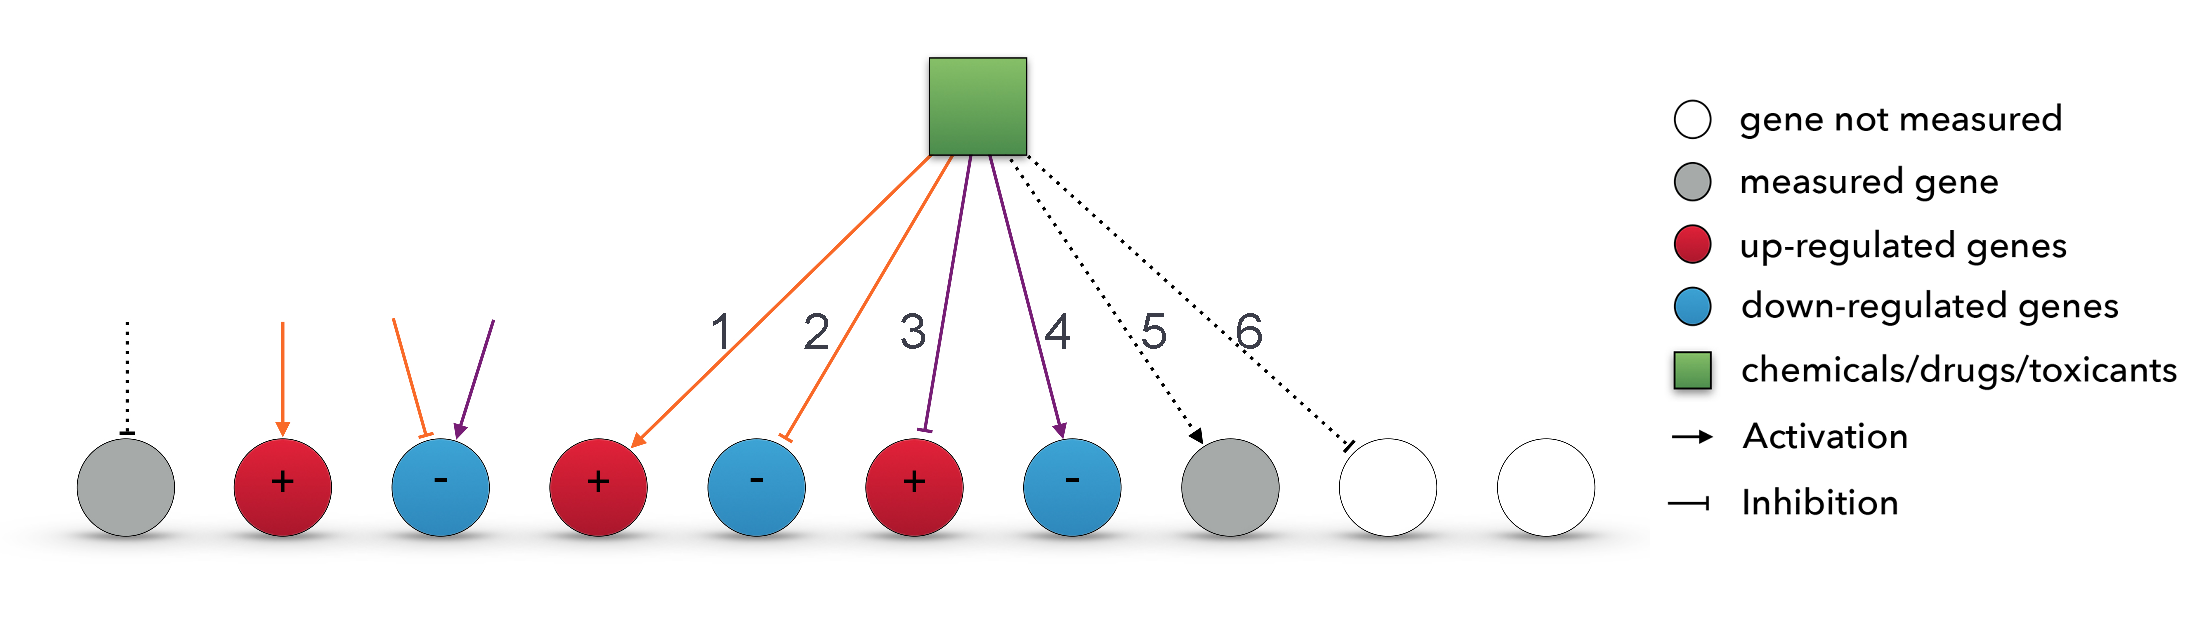
\includegraphics[width=0.9\linewidth]{Figures/SecondEvidence.pdf}
  \caption{Illustration of different types of genes available in the Comparative Toxicogenomics Database and gene expression profile, and their relationships with the chemical. The significance of a chemical/drug/toxicant (green box) in each hypothesis is assessed using a statistical test based on the number of up- or down-regulated DE genes and their associations with the drug. The orange edges (e.g. 1 and 2) are the ones that support the hypothesis that level of studied chemical/drug/toxicant is higher in the phenotype compared to the control while the purple ones (e.g. 3 and 4) are supporting the hypothesis that its level is lower compared to the control.}
  \label{fig:SignificantDrug}
\end{figure*}

We define G as  the set of genes included in both $G_{DE}$ and $G_{KB}$, i.e.  $G_{DE} \cap G_{KB}$. Subsequently, $C \subseteq C_{KB}$  and $E \subseteq E_{KB}$ represent the set of all CDTs and their corresponding associations with those genes in $G$ available in the knowledge base. These sets are formally defined as follows:

\begin{equation}C = \{c \in C_{KB} \mid \exists g \in G \land \exists e_{c,g} \in E_{KB} \}\end{equation}

and 

\begin{equation} E = \{ e_{c,g} \mid \exists c \in C \land  \exists g \in G \ \land  e_{c,g} \in E_{KB} \} \end{equation}

%Let $G^{+}\subseteq G$ and $G^{-}\subseteq G$ be the list of up- and down-regulated DE genes, respectively. 

where $e_{c,g}$ denotes an edge from an upstream CDTs $c$ to targeted gene $g$ representing their relationship described in the Comparative Toxicogenomics Database. The sign of the edge, $s(e_{c,g})$, reflects the type of the association, namely positive ($+$) for an activation and negative ($-$) for an inhibition edge. Also, we denote $s(g)$ the sign of the DE gene $g$ which is positive if $g$ is up-regulated, and negative, otherwise. 

Each edge $e \in E$ is labeled whether it is supporting either of the testing hypotheses (Fig.~\ref{fig:SignificantDrug}). 
For example, if an edge is activation and its targeted DE gene is indeed up-regulated, the edge supports the hypothesis 1. 
%Similarly, an inhibition edge connected with a down-regulated DE gene is also backing this hypothesis. 
In essence, an edge is considered to be supporting the hypothesis 1 when its sign, $s(e_{c,x})$, is aligned with the sign of its targeted DE gene, namely $s(e_{c,g}) = s(g)$. 
Such edges are colored orange in Fig.~\ref{fig:SignificantDrug}. 
Edges whose signs are opposite with the expression direction of their targeted DE genes are considered as a supporting evidence for the hypothesis 2, and are colored purple in  Fig.~\ref{fig:SignificantDrug}. 
Notice that $E^{H1}$ and $E^{H2}$ are the two mutually exclusive sets of edges that support the first and second hypothesis, respectively, because an edge $e \in E$ must support either the hypothesis 1 or hypothesis 2, but not both. Formally, $E^{H1} \cap E^{H2} = \emptyset$ and  $E^{H1} \cup E^{H2} = E$. 

For each chemical $c \in C$, a statistical score, i.e. p value, for each aforementioned hypothesis is then computed using the one-sided Fisher's exact test. Without losing generality, let us discuss the hypothesis 1. First, a confusion matrix is constructed as in Table \ref{ConfusionMatrix}, where $l$, $k$, $m$, and $n$ are the number of edges related to $c$ that support the hypothesis, the number of edges related to $c$ that do not support the hypothesis, the number of edges not related to $c$ that support the hypothesis, and the number of edges not related to $c$ that do not support the hypothesis, respectively. 
The probability of this observed contingency under the null hypothesis is defined as follows:
\begin{equation}
p = \frac{ {l+k \choose l}{m+n \choose m}}{{\|E\| \choose l + m}}
\end{equation}
where $\|E\| = (l+k+m+n)$ is the number all edges in $E$. 

The p value of the one-sided Fisher's exact test is the sum of the probabilities of all contingency tables that have the number of edges supporting the H1 more than $l$ where the number of edges related to the compound C and the number of edges supporting the H1 are unchanged.

Notice that because an edge supporting H1 is against H2 and vice versa, the contingency matrix for H2 can be obtained by swapping the columns of the observed contingency matrix of H1. Hence, the p value for the H2 can also be derived from these four numbers.


Finally, we use the false discovery rate (FDR) to correct the p values for multiple comparisons~\cite{Benjamini:1997}.

\begin{table}
\caption{For each chemical/drug/toxicant $c$, a contingency table is constructed. Here, \emph{l}, \emph{k}, \emph{m}, and \emph{n} are the number of edges coming from $c$ that support the hypothesis 1 (H1), the number of edges coming from $c$ that do not support the H1, the number of edges not coming from $c$ that support the H1, and the number of edges not coming from $c$ that do not support the H1, respectively. Note that the edges that support H1 are against the hypothesis 2 (H2), and vice versa. Hence, a similar contingency table for H2 can be constructed using these four numbers.}
\begin{center}
\begin{tabular}{c|cc}
&  Supporting H1& Against H1\\
\hline
Related to $c$& \emph{l} & \emph{k} \\
 Not related to $c$&\emph{m}& \emph{n}  \\
%\hline 
%Total & $\|E1\|$ & $\|E2\|$ & $\|E\|$
\end{tabular}
\end{center}
\label{ConfusionMatrix}
\end{table}%


\subsection{Assessment}

We evaluate and compare the performance of our proposed method with the other five approaches, namely Over Representation Analysis (ORA) using hypergeometric test, Kolmogorov-Smirnov test (KS)\cite{massey1951kolmogorov}, Wilcoxon\cite{wilcoxon1945individual}, FGSEA~\cite{korotkevich2021fast}, and the causal analysis used in Ingenuity Pathway Analysis (IPA)~\cite{kramer2013causal}.


\subsubsection{Benchmarking methods}

The ORA family of methods, as well as other tests, such as KS, Wilcoxon, and FGSEA, are widely used in gene set analysis to determine whether  a particular gene set - such as the genes associated to a given GO term or pathway - is significantly affected in the given phenotype. In principle, the same approach could be used to decide whether a given CDT could be related to the phenotype by considering the set of genes known to be affected by the given CDT. 

\textbf{ORA} uses a statistical test, such as hypergeometric, chi-square, or binomial distribution, to evaluate if the number of DE genes is over- or under-represented in the set of targeted genes of a CDT. In this study, we use hypergeometric test to compute p value, namely the probability of getting the $x$ or more observed DE genes in $M$ CDT's downstream genes from a pool of $N$ background genes with $n$ DE genes. Mathematically, this probability is defined as:

\begin{equation*}
P(X \geq x) = 1-P(X \leq x -1)= 1- \sum_{i=0}^{x-1} \frac{\binom{M}{i}\binom{N-M}{n-i}}{\binom{N}{n}} 
\end{equation*}

ORA does not take into consideration if the DE gene is up-regulated or down-regulated, nor the type of associations between the CDT and the targeted DE gene.

The Kolmogorov-Smirnov test (\textbf{KS}) determines whether there is a significantly difference between two empirical distributions of the scores (the direction of the fold changes) of the DE genes targeted by the CDT (\texttt{DEhit}) and those of the DE genes not targeted by the CDT (\texttt{DEmiss}). First, all genes will be ranked in order of their log fold changes. Then, we calculate the cumulative distribution function (CDF) of the ranked gene list for background genes and for the genes affected by the CDT. Finally, the KS test is used to compare the two CDFs and calculates a p value that measures the significance of the enrichment. Although KS takes the sign of the DE genes into consideration (the fold changes of gene expression), it ignores the type of associations between CDTs and DE genes.

\textbf{Wilcoxon} is a rank-based non-parametric test for comparing the ranks of DE genes affected by the CDT (\texttt{DEhit}), and other DE genes (\texttt{DEmiss}). First, it ranks all genes in both lists based on their fold changes. Subsequently, it computes the a test statistic $W$, which is the sum of the ranks for all \texttt{DEhit}. This test statistic $W$ is compared to the distribution of $W$ under the null hypothesis. The null hypothesis is rejected if $W$ is extreme and falls outside 95\% of the distribution. In R, the Wilcoxon is available via the function \texttt{wilcox.test}.  Similar to ORA, the  associations of the affected DE genes with the CDT are completely ignored.

\textbf{FGSEA} is an improvement of the Gene Set Enrichment Analysis (GSEA) approach. FGSEA accelerates the calculation of the GSEA p value by estimating it with a high accuracy (the estimation error is less than $10^{-100}$ when compared with actual GSEA p value). GSEA, in turn, is one of the most popular approaches in gene set analysis\cite{Subramanian:2005}. It consists of three important steps: computing the enrichment score for each gene set, estimating the statistical significance of the enrichment score, and adjusting for multiple hypothesis testing. We used the function \texttt{fgsea} in the ``fgsea'' package with the parameters \texttt{nperm = 10\textsuperscript{4}} and \texttt{minSize = 15}.

\textbf{IPA} is a commercial web-based platform that offers several applications including a causal analysis tool\cite{kramer2013causal}. Given a list of DE genes, IPA's causal analysis outputs a list of upstream regulators including chemicals/drugs, as well as genes, proteins families, complexes, microRNA, and biological processes.
Notice that including all these types of regulators in the report would worsen the IPA's result when benchmarking with other methods since it might increase the rank of the true CDT. Moreover, since there is only one true causal CDT in each experiment and all other elements are considered as false positives, having them in the result would increase the number of false positives. 
For these reasons, beside the default IPA result, we added to the method benchmarking the so-called IPA-CDT  that only retains the CDTs in the IPA report and excludes all non-chemical elements.

According to Kr\"{a}mer \textit{et al.}, IPA derives two scores for each regulator \textit{r}, namely the overlap p-value and the activation z-score, as follows.

\emph{The overlap p-value} reflects the enrichment of the list of \textit{r}-regulated genes in the set of all DE genes without taking the regulation direction into consideration. Formally, it is based on the one-sided Fisher's exact test and is calculated as follows:

\begin{equation*}
p(r)=\sum_{k = 0}^{min(c,d)} \frac{(a+b)!(c+d)!(a+c)!(b+d)!}{(a+k)!(b-k)!(c-k)!(d+k)!n!}
\end{equation*}

where $n$ is the number of all background genes, i.e. all the genes in the data set that have at least one association with any upstream regulator, $a$ is the number of DE genes regulated by $r$, $b$ is the number of DE genes that are not regulated by $r$, $c$ is the number of $r$-regulated genes but not differentially expressed, and $d=n-a-b-c$.

\emph{The activation z-score} uses the information about the direction of gene regulation to predict the regulators. Let $\tilde{O}$ be the set of $r$-regulated DE genes, the activation z-score of the corresponding regulator $r$ is defined as:


\begin{equation*}
z(r) =  \frac{\sum\limits_{v \in \tilde{O}}w_{R}(r,v) s_{R}(r,v) s_{D}(v)}{\left(\sum\limits_{v \in \tilde{O}}[w_{R}(r,v)]^2\right)^{1/2}}
\end{equation*}

where $w_{R}(r,v)$ represents the weight associated with the regulation of $r$ and the downstream DE gene $v$, $s_{R}(r,v)$ is the sign of the regulation, i.e. $s_{R}(r,v)=1$ for activation and $s_{R}(r,v)=-1$ for inhibition, and $s_{D}(v)$ represents the direction of DE gene's expression, i.e. $s_{D}(v)=1$ for up-regulation and $s_{D}(v)=-1$ for down-regulation, respectively. The activation z-score is proven to be approximately normally distributed under the null model, e.g. random signs $s_{R}(r,v)$ and $s_{D}(v)$. On one hand, a high positive z-score, e.g. $z(r) > 2$, indicates that the match between the signs of downstream DE genes ($s_{D}(v)$) and the corresponding edges ($s_{R}(r,v)$) is significant, which in turn suggests that $r$ is the activated regulator. On the other hand, a low negative z-score, e.g. $z(r) <  -2$, is an indicator that the sign of the downstream DE genes are mostly opposite with the corresponding regulations. In this case, $r$ is predicted as an inhibitor~\cite{kramer2013causal}.



Among all the benchmarking methods included in this study, only IPA takes the sign of CDTs - genes associations under consideration and can predict whether a significant CDTs is activated or inhibited (corresponding to H1 and H2), as PURE does, so a more detailed theoretical comparison is warranted.
Although IPA derives these two scores  described above for each CDT, the result is solely determined by the z-score: the regulator is determined as ``activated''  or ``inhibited'' if its z-score $\geq 2$ or $\leq -2$, respectively~\cite{kramer2013causal}. In other words, the statistic calculated from the data will determine the outcome. In contrast, PURE uses a more classical approach in which the hypotheses are formulated before hand, independently of the data as in a canonical hypothesis testing. PURE considers each hypothesis separately, and calculates a p-value that will indicate whether the null hypothesis can be rejected. 
For PURE, the null hypothesis is that ``CDT X has not had an impact on the measured gene expression changes" whereas the first research hypothesis is that ``CTD X was present and had an impact on the gene expression changes'' and the second, independent, research hypothesis is that ``CTD X was lacking and its absence had an impact on the gene expression changes''. 
The testing done in the proposed approach is more rigorous in terms of statistical testing, but such approach can potentially reject the null hypothesis for both research hypotheses which would be difficult to interpret from a biological perspective. In contrast, the approach used by IPA avoids such potentially ambiguous situations because the z-score can be either positive or negative but not both. The most important difference stemming from these two approaches is that PURE can identify CDTs that can reverse the observed genes expression changes because it considers both sets of statistical hypothesis. This means that PURE can be used for drug repurposing - situations in which one is given a   gene expression profile associated with a given disease and the task is to identify a drug that could revert some of the changes. In contrast, IPA only considers the CDTs that are present and focuses whether they are ``activated'' or ``inhibited''. 
Another  difference worth mentioning between IPA and PURE is that while PURE considers and derives a p value corresponding to the hypothesis testing for every CDT in the knowledge base, IPA does not derive z-score for all CDT in the knowledge base. %For example, Methylprednisolone is in the IPA's knowledge base and has z-score in the experiment 15, but no z-score is reported in the experiment 16 (Table ~\ref{H2Result}).

\subsection*{Testing Hypothesis 1}
We evaluate these methods using 14 benchmark data sets from three different species, namely human, mouse, and rat (See Table \ref{Datasets}). 
In these data sets, gene expressions were measured after the ingestion of a given CDT.
Hence, the cause of all the changes observed  throughout the system is known. Furthermore, this particular situation corresponds to  H1, where the level of the CDT is higher than normal.
We consider the administered CDT as the ``true CDT'' for each of these data sets.

The result of each method is a ranked list of CDTs based on the particular statistic used by each method, i.e. FDR-adjusted p values for PURE, ORA, KS, Wilcoxon, and FGSEA, and  z-score  for IPA and IPA-CDT. 
If several CDTs are ranked with the same statistic, we use an average. For instance, if  the top 4 elements have the same p value, they would be all ranked as 2.5 instead of 1, 2, 3, and 4, respectively because 2.5 is the average of the set $\{1, 2, 3, 4\}$.
An ideal method would be able to identify the true CDT by ranking it on top with a significant p value $\leq 0.05$ or  z-score $\geq 2$ (or z-score $\leq -2$ in case of IPA testing the H2).

%There are 14 data sets corresponding to the H1 where the causal CDTs are known (Table~\ref{Datasets}). We report and compare the ranks of the true CDTs in these 14 data sets (see Table~\ref{Ranks} and Fig.~\ref{fig:resultFigure}a).
%PURE (average = 2.8) is better than all of the methods in this study, followed by IPA-CDT (average = 17.7), ORA (average = 20.1), and KS (average = 24), GSEA (average = 32.9), IPA (average = 79.9), and Wilcoxon (average = 104.4) (Table \ref{Ranks}). PURE can successfully identify the true CDTs in these 14 benchmarking data sets and rank them at the top 7 times. It performs better than all of the methods in 9 data sets. IPA-CDT performs best in 6 data sets (3 of which are tied with PURE) and is able to rank the true CDTs at the top 5 times. However, it cannot identify the true CDTs in three data sets, in two of which the true CDTs are not present in the result list (data set 8 and data set 14). Similar to IPA-CDT, IPA can correctly rank the true CDTs at the top in 5 data sets.  FGSEA performs best in 2 data sets. ORA performs best in one data sets (tied with PURE), while KS and Wilcoxon are not able to perform best in any of the experiment.


However, an evaluation based solely on the method's ability to identify the true CDT using the p value does not show the whole story and sometimes misleads.
For example, a method that derives low p values for all CDTs can always identify the true CDT, but is still considered a bad one because it includes a lot of false positives in the result.
Therefore, we also take the number of false positives in the result into consideration, i.e. the number of CDTs that are not true CDT but reported as significant. % (Fig. \ref{fig:resultFigure}b).
Although chemicals and drugs could have similar effects or could be in the same family, we only consider the true CDT as the one and only true positive and all other CDTs as true negatives.
We expect a good method would derive a low number of CDTs in the result, ideally only one, the true CDT.
%Our method generally reports the lower numbers of reported chemicals (average = 19.4) than any other methods compared, followed by FGSEA (average = 37.4) and IPA-CDT (average = 37.6).
%Although FGSEA is comparable to IPA-CDT, it cannot identify the true CDTs in 6 out of 14 experiments while IPA  cannot identify only 3 out of 15.
%Wilcoxon and IPA report on average more than 100 CDTs while ORA and KS report on average more than 200 CDTs per experiment (Table \ref{NrSig}).

To investigate whether or not  PURE is superior to the other methods, we used a Wilcoxon test to compare the ranks and number of CDTs reported by PURE with those provided by the  other methods. 
%The p values for the rank comparison of PURE and IPA-CDT, ORA, KS, FGSEA, IPA, and Wilcoxon are 0.02, 4E-4, 8E-6, 4E-5, 6E-3, and 1E-5, respectively. 
If the rank of the true CDTs is not available in an experiment, we replace the NA ranks by the number of significant CDTs reported in the corresponding experiment plus one, 
e.g. if a method reports a list of 30 significant CDTs but the true CDTs is not included, we assigned 31 to the true CDT's rank.
%e.g in the experiment 9 performed by IPA, we assigned 31 to the true CDT's rank because IPA reported a list of 30 significant CDTs but the true CDTs is not included (Table ~\ref{NrSig}). 
%The p value for the number of CDTs reported comparison between PURE and IPA-CDT, ORA, KS,  FGSEA, IPA, and Wilcoxon are 0.04, 4E-4, 9E-6, 0.4, 4E-5, and 2E-6, respectively. 
%Since all  p values are less than the standard threshold of 0.05 (except for FGSEA while comparing the number of CDTs reported), PURE's performance can be considered significantly better than all of the methods included in the study, in terms of both the rank of the true CDTs, as well as the number of significant CDTs reported.

\subsubsection{Testing Hypothesis 2}

The assessment of these methods on testing H2 is more challenging since the data sets in which the ground truth is known are scant, i.e. an CDT is truly lacking in the system. Another important application for testing the H2 is drug repurposing. A CDT could potentially reverse the  gene expression changes caused by the disease and therefore be a candidate for drug repurposing. 
%Similar approach using the data set GSE147507, in which the expression of NHBE and A549 cells infected with COVID-19 were compared with their corresponding control, proposed Methylprednisolone to improve the outcome in server COVID-19 cases~\cite{DraghiciCOVID:2021}. This finding was aligned with several clinical trials from different research groups~\cite{DraghiciCOVID:2021, corral2021methylprednisolone,salton2020prolonged, meduri2020pharmacological}. 
At the time we applied PURE to the COVID-19 data, the recommendation of several organizations, including the World Health Organization (WHO), CDC, and Surviving Sepsis Campaign, was against the use of any systemic corticosteroids in the severe cases of COVID-19~\cite{wilson2020covid}. 
%Surprisingly, our results showed that Methylprednisolone, a corticosteroid, would be effective in helping the patients with severe disease~\cite{DraghiciCOVID:2021}. 
Subsequently, clinical trials have shown that indeed steroids are effective and the world health organization has reversed their recommendation\cite{meduri2020pharmacological, corral2021methylprednisolone,salton2020prolonged, meduri2020pharmacological, cochrane1996systemic, prescott2020corticosteroids}. At this time, the standard of care in severe cases of COVID-19 is the corticosteroid treatment. 
Hence, in this study, we use the data set GSE147507 in which the expression of NHBE and A549 cells infected with COVID-19 were compared with their corresponding control, and consider Methylprednisolone as the ``target'' CDT in the experiments 15 and 16 for different contrasts. %(Table~\ref{H2Result}).

We evaluate the methods' performance based on the same criteria: rank of the target CDT (Methylprednisolone), and the number of CDTs reported. 
%Our proposed method, PURE, is able to identify Methylprednisolone in both experiments with the average rank of 3.25, followed by FGSEA (average = 6.5), ORA (average = 14.75), KS (average = 19.5), Wilcoxon (average = 29), IPA-CDT (average = 393), and IPA (average = 890). Notice that although ORA, KS, Wilcoxon, and FGSEA can identify Methylprednisolone as significant CDT, they cannot determine whether it is present or absent. Also, IPA cannot identify Methylprednisolone in either experiments. More importantly, all other methods, except for FGSEA, reported hundreds of significant CDTs in each experiment, which make it difficult for a researcher to identify a truly effective drug such as Methylprednisolone. Hence, in term of number of CDTs reported, PURE also performs better than other methods. The average number of CDTs reported by PURE is 10 CDTs, whereas that number of FGSEA, IPA-CDT, Wilcoxon, KS, IPA, ORA are 27.5, 103, 189, 216, 238, 553, respectively (Table~\ref{H2Result}). 
Since the sample size is small (only 2 experiments), we do not compute p values for these comparisons.

%PURE can identify the true CDTs in all of the experiments.
%Also notice that in data set 13, IPA could determine the target chemical, dexamethasone, as significant and rank it 13, there are 173 other false positive chemicals in the result.
%

%
%\begin{table}
%\caption{\label{Ranks} Benchmarking the methods in term of the ranks of the true CDTs. The experiment IDs (Exp. ID) are corresponding to the ones in Table \ref{Datasets}. The lower the rank of the true CDTs, the better.  The green highlighted cell is the best one in each experiment. PURE performs best in 9 out of 14 experiments, followed by IPA which performs best in 6 experiments (3 co-best with PURE). In two of the data sets analyzed IPA was not able to identify the correct CDT at all  (highlighted in red).}
%\begin{center}
%\scriptsize
%\begin{tabular}{ ccc|ccccccc } 
%
% \hline \hline
%
%\multirow{2}{*}{Exp. ID}& \multirow{2}{*}{GEO ID}& \multirow{2}{*}{Organism} & \multicolumn{7}{c}{\textbf{Rank of true CDTs}} \\
%&  && PURE  & ORA & KS  & Wilcoxon & FGSEA & IPA& IPA-CDT\\
%\hline
%1	& GSE26487& Human &	\cellcolor{green}1	&	1.5	&	43	&	45	&	25.5	& \cellcolor{green}1&	\cellcolor{green}1\\ 
%
%2	& GSE49804& Mouse	&	2	&	2	&	33	&	11	&	16.5	&	\cellcolor{green}1 & \cellcolor{green}1\\ 
%
%3	& GSE86837& Mouse	&	\cellcolor{green}1	&	\cellcolor{green}1	&	3	&	2.5	&	47	&	816& 153\\ 
%
%4	& GSE58434\_H& Human &	\cellcolor{green}1	&	16	&	13.5	&	65	&	159	&	25 & 14\\ 
%
%5	& GSE58434\_Ast& Human &	\cellcolor{green}2	&	18	&	23.5	&	254	&	30.5	&	26 & 5\\ 
%
%6	& GSE11352\_12h & Human	&	\cellcolor{green}1	&	32.5	&	24.5	&	126	&	4.5	&	\cellcolor{green}1 & \cellcolor{green}1\\ 
%
%7	& GSE11352\_24h & Human	&	\cellcolor{green}1	&	33	&	24	&	214	&	7.5	&	\cellcolor{green}1 & \cellcolor{green}1\\ 
%
%8	& GSE11352\_48h & Human	&	2	&	29.5	&	24	&	153	&	24.5	&	\cellcolor{green}1 & \cellcolor{green}1\\ 
%
%9	& GSE74000 & Human	&	\cellcolor{green}1	&	16	&	23	&	9	&	75	&	\cellcolor{red}NA & \cellcolor{red}NA\\ 
%
%10	& GSE12446\_WT & Human	&	4	&	31	&	39.5	&	460.5	&	27.5	& 10 & 	\cellcolor{green}3\\ 
%
%11	& GSE67266\_KO	& Mouse	&	6	&	22	&	27	&	32	&	\cellcolor{green}3.5	&	22 & 12\\ 
%
%12	& GSE67266&	Mouse	&	7.5	&	25	&	38	&	62.5	&	\cellcolor{green}2.5	&	21 & 7\\ 
%
%13	& GSE51213	& Mouse	&	\cellcolor{green}9	&	52	&	18	&	26	&	33	&	34 & 13\\ 
%
%14	& GSE58875	& Rat 	&	\cellcolor{green}1	&	1.5	&	1.5	&	1.5	&	3	&	\cellcolor{red}NA & \cellcolor{red}NA\\ 
% \hline \hline
% \multicolumn{3}{c}{Average $\pm$ std. dev. }	 &\cellcolor{green} \makecell{2.8\\ $\pm$ 2.7 }	&	 \makecell{20.1\\ $\pm$ 15.2  }	&	 \makecell{24.0\\ $\pm$  12.3}	&	 \makecell{104.5\\ $\pm$    130.4 }	&	 \makecell{ 32.8 \\ $\pm$  41.5 }&	 \makecell{79.9\\ $\pm$ 232.1  }&  \makecell{17.7\\ $\pm$  42.9}\\ 
%
%\end{tabular}
%
%\end{center}
%\end{table}

%
%\begin{table}
%\caption{\label{NrSig} Benchmarking the methods in term of the number of significant CDTs reported. The experiment IDs (Exp. ID) are corresponding to the ones in Table \ref{Datasets}. The cell is highlighted green if the number of reported CDTs less than 10; blue if  it is more than or equal to 10 but less than or equal 20. The cell is highlighted red if the true CDT is not included at all in the reported list of significant CDTs by the method (i.e. all reported CDTs are false positives). For instance, in the first row PURE only reported only one CDT and that was the correct one (zero false positives). Hence, PURE's cell is colored green. FGSEA  reported two significant CDTs but the cell is colored red because the reported CDTs are a false positives. The true CDT was  not significant and was ranked 25.5 (Table ~\ref{Ranks}). In the same data set, IPA-CDT ranked the true CDT first (Table ~\ref{Ranks}). However, the cell is colored blue because it also included 13 other CDTs which are considered false positives.}
%\begin{center}
%\scriptsize
%\begin{tabular}{ ccc|cccccccc } 
%
% \hline \hline
%
%\multirow{2}{*}{Exp. ID}& \multirow{2}{*}{GEO ID}& \multirow{2}{*}{Organism}& \multicolumn{7}{c}{\textbf{Number of significant CDTs reported}} \\
%& & &   PURE  & ORA & KS  & Wilcoxon & FGSEA & IPA & IPA-CDT\\
%\hline
%1	& GSE26487& Human &	\cellcolor{green}1	&	58	&	117	&	45	&	\cellcolor{red}2	& 23 &	\cellcolor{cyan}14\\
%2	& GSE49804& Mouse	&	\cellcolor{green}4	&	\cellcolor{cyan}14	&	67	&	47	&	\cellcolor{red}0	&	\cellcolor{cyan}18 & \cellcolor{cyan}10\\
%3	& GSE86837& Mouse	&	\cellcolor{green}1	&	93	&	104	&	77	&	\cellcolor{red}0	& \cellcolor{red}191 &	\cellcolor{red}14\\
%4	& GSE58434\_H& Human &		\cellcolor{cyan}13	&	703	&	257	&	167	&	\cellcolor{red}89 &	170 &	75\\
%5	& GSE58434\_Ast& Human &	\cellcolor{green}8	&	520	&	267	&	\cellcolor{red}154	&	\cellcolor{red}19	& 199 &	35\\
%6	& GSE11352\_12h & Human	&	28	&	376	&	299	&	\cellcolor{red}123	&	\cellcolor{cyan}18	& 79&	\cellcolor{green}6\\
%7	& GSE11352\_24h & Human	&	25	&	384	&	325	&	\cellcolor{red}154	&	32	&125 &	\cellcolor{cyan}13\\
%8	& GSE11352\_48h & Human	&	31	&	369	&	304	&	\cellcolor{red}131	&	62	&324 & 	22\\
%9	& GSE74000 & Human	&	\cellcolor{cyan}17	&	248	&	300	&	82	&	\cellcolor{red}7	&	\cellcolor{red}30 & \cellcolor{red}14\\
%10	& GSE12446\_WT & Human	&	33	&	297	&	494	&	\cellcolor{red}236	&	139	&	226 & 31\\
%11	& GSE67266\_KO	& Mouse	&	\cellcolor{cyan}20	&	118	&	116	&	70	&	\cellcolor{cyan}10	&	156& 61\\
%12	& GSE67266&	Mouse	&	22	&	96	&	118	&	91	&	\cellcolor{cyan}13	& 341&	53\\
%13	& GSE51213	& Mouse	&	66	&	184	&	331	&	254	&	133	&	533& 174\\
%14	& GSE58875	& Rat 	&	\cellcolor{green}2	&	\cellcolor{green}2	&	\cellcolor{green}2	&	27	&	\cellcolor{red}0	&\cellcolor{red}16&	\cellcolor{red}5\\
%\hline
%\multicolumn{3}{c}{Average $\pm$ std. dev. }& \makecell{19.4 \\$\pm$ 17.5 } & \makecell{247.3 \\$\pm$ 206.1} & \makecell{221.5 \\$\pm$ 135.3} & \makecell{118.4 \\$\pm$  69.2} & \makecell{37.4 \\$\pm$ 49} & \makecell{173.6 \\$\pm$ 148.7} & \makecell{37.6 \\$\pm$ 44.9} \\ \hline \hline
% 
%\end{tabular}
%\end{center}
%\end{table}

%
%\begin{table}
%\caption{\label{H2Result} Benchmarking the methods for accepting the H2. Green highlighted cells are best for each row. Red highlighted cells indicate that the target CDTs are not included in the reported list. Notice that ORA, KS, Wilcoxon, and FGSEA reject the null hypothesis and identify the target CDTs as significant to the observed changes in the gene expression profiles, they do not distinguish the two hypotheses H1 and H2. Beside PURE and FGSEA, all other methods include more than hundred CDTs in the significant lists.}
%\begin{center}
%\scriptsize
%\begin{tabular}{ ccc|cccccccc } 
%
% \hline \hline
%
%\multirow{2}{*}{Exp. ID}& \multirow{2}{*}{GEO ID}& \multirow{2}{*}{Organism}& \multicolumn{7}{c}{\textbf{Rank of true CDTs}} \\
%& & &   PURE  & ORA & KS  & Wilcoxon & FGSEA & IPA & IPA-CDT\\
%\hline
%15	& GSE147507\_NHBE	& Human	&	\cellcolor{green}2.5	&	23	&	12	&	24	&	8.5	&	\cellcolor{red}890 &\cellcolor{red} 393\\
%16	& GSE147507\_A549	& Human 	&	\cellcolor{green}4	&	6.5	&	27	&	34	&	4.5	& \cellcolor{red}NA & \cellcolor{red}NA\\
%\hline
%\multicolumn{3}{c}{Average}	& 	\cellcolor{green}3.25 	&	14.75	 & 	19.5 	& 	29 	& 	6.5 	& 	890 	&	393 \\ 
%\hline 
% \multicolumn{10}{c}{}\\
%\hline
%
%
%\multirow{2}{*}{Exp. ID}& \multirow{2}{*}{GEO ID}& \multirow{2}{*}{Organism}& \multicolumn{7}{c}{\textbf{Number of significant CDTs reported}} \\
%& & &   PURE  & ORA & KS  & Wilcoxon & FGSEA & IPA & IPA-CDT\\
%
%\hline
%15	& GSE147507\_NHBE	& Human	&	\cellcolor{green}8	&	719	&	274	&	224	&	40	&	\cellcolor{red}371& 	\cellcolor{red}182\\
%16	& GSE147507\_A549	& Human 	&	\cellcolor{green}12	&	387	&	159	&	154	& 	15 	& 	\cellcolor{red}105&		\cellcolor{red}24\\
%\hline
%\multicolumn{3}{c}{Average}& \cellcolor{green}10 &	553 	&	216 	& 189 	& 	27.5 & 238 & 103 \\ 
%\hline \hline
% 
%\end{tabular}
%\end{center}
%\end{table}
%
%
%\begin{figure*}
%\begin{center}
%%\includegraphics[width=0.49\linewidth]{Figures/RankTarget_v4.pdf}
%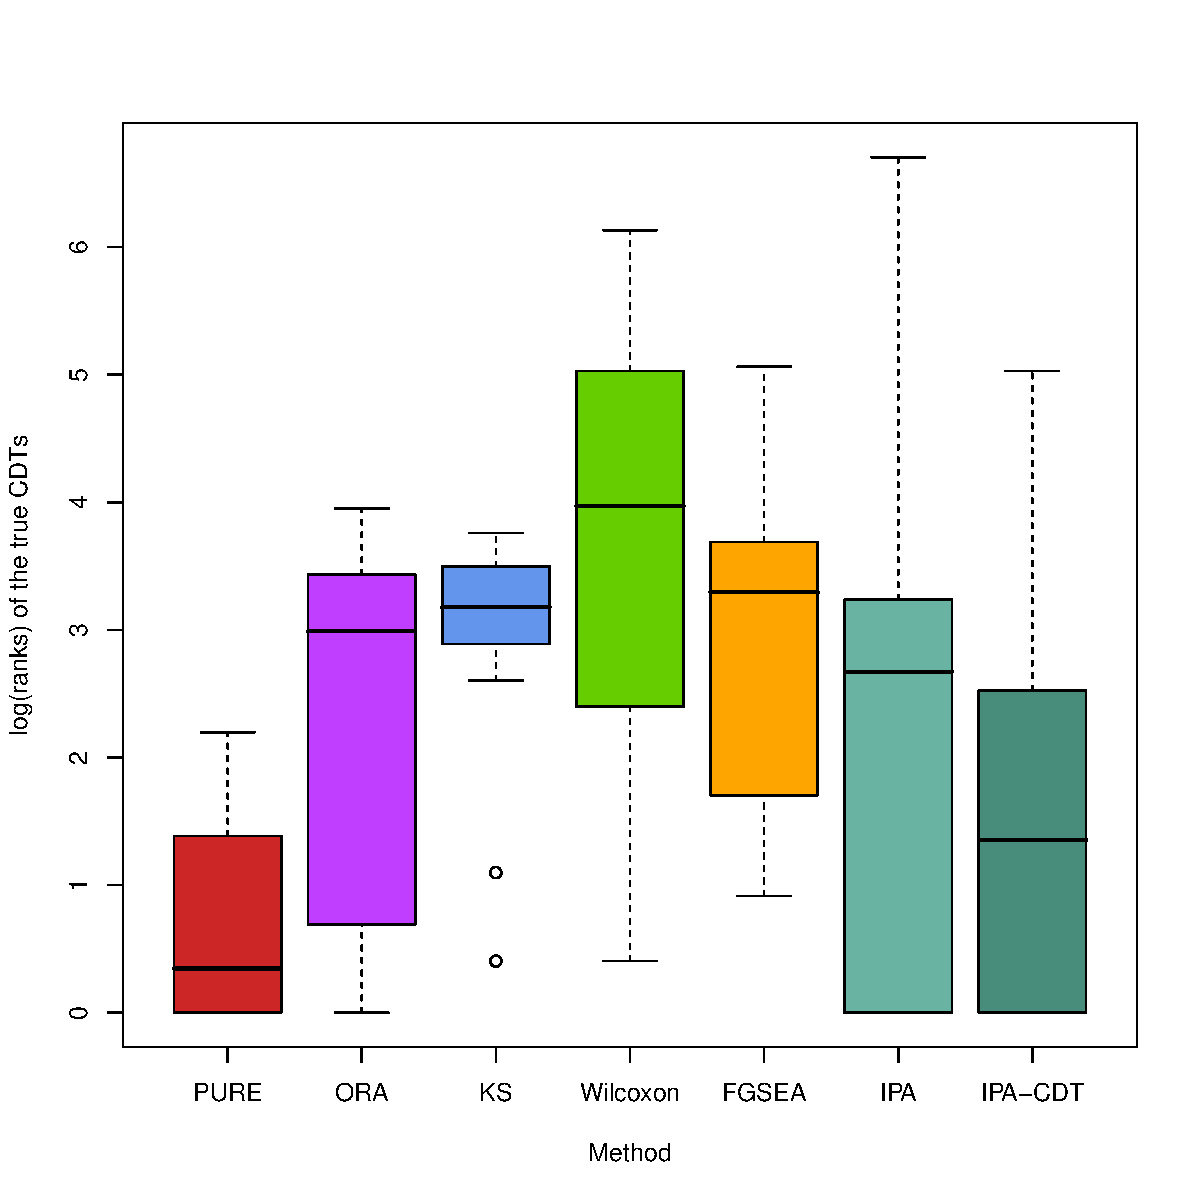
\includegraphics[width=0.49\linewidth]{Figures/RankTarget_vOrg_log.pdf}
%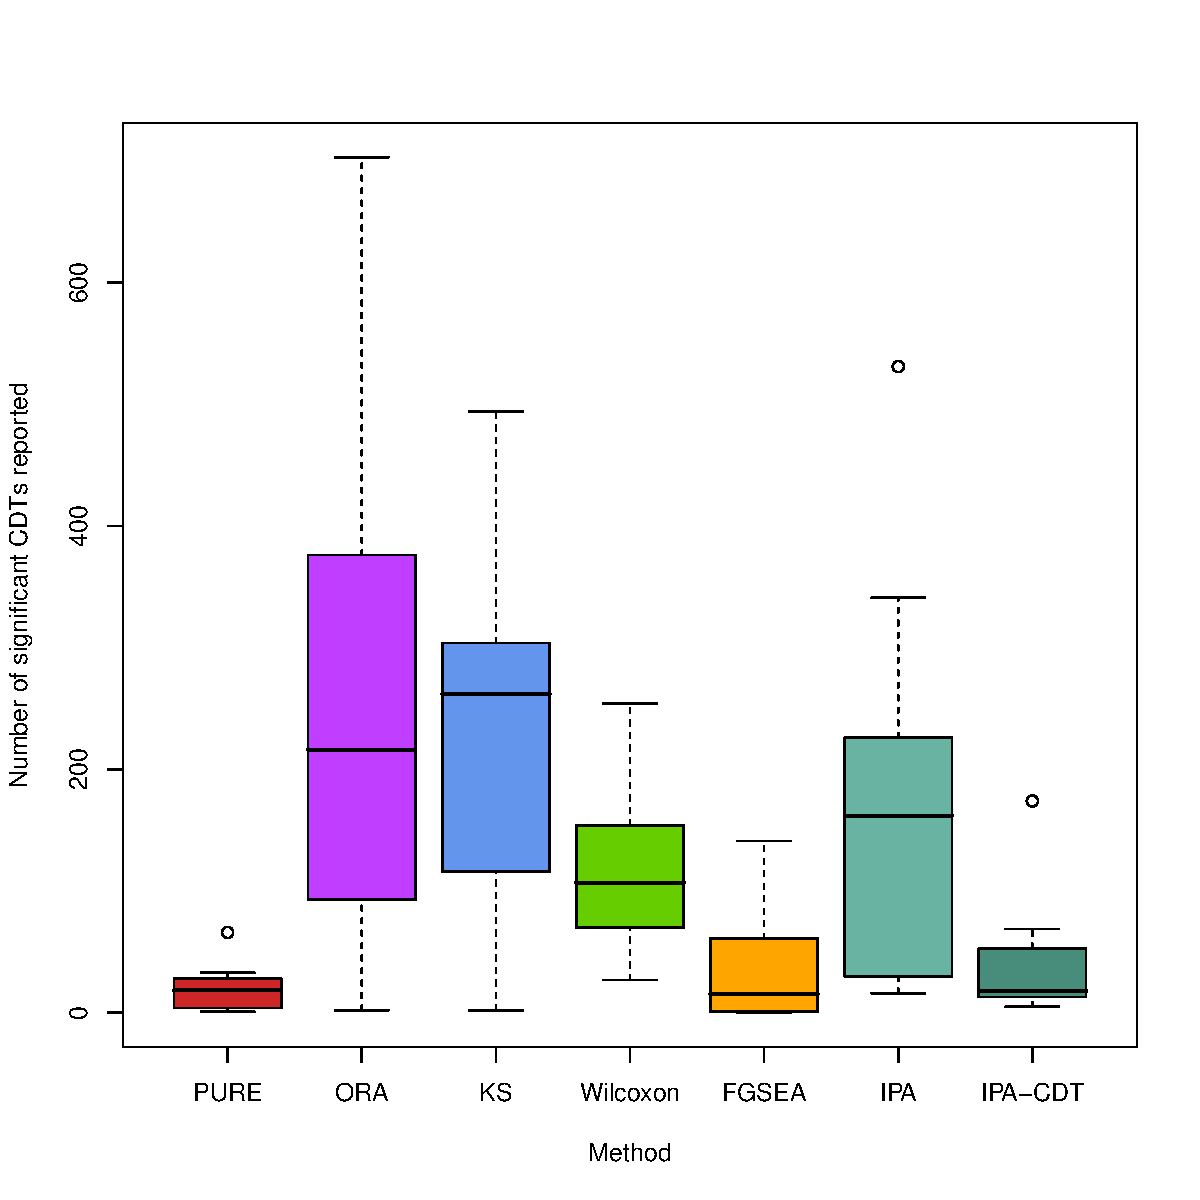
\includegraphics[width=0.49\linewidth]{Figures/NrSigChem_vOrg.pdf}
%%\includegraphics[width=0.32\linewidth]{Figures/pValueTarget_v2.pdf}
%
%\caption{The comparison of PURE and other 5 methods, in term of log(ranks) of true CDTs (left panel) and the number of significant chemicals reported (right panel). In the left panel, a better method would rank the true CDT as low as possible (ideally rank it 1) so lower log(rank) values are better. A CDT that is different from the true CDT and yet reported as significant is a false positive. For this reason, we would like the number of CDTs reported as significant (shown in the right panel) to also be as low as possible. }
%\label{fig:resultFigure}
%\end{center}
%\end{figure*}

\subsection{Discussion}

In this manuscript, we propose PURE, a causal analysis approach that infers the CDTs responsible for the changes in the gene expression profile, either because their level in the subject's system is higher (hypothesis 1) or lower (hypothesis 2) than normal. 
%This application is a crucial step to treat conditions related to external CDTs since it helps identifying the correct causal CDTs causing observed list of DE genes. 
On one hand,  hypothesis 1 helps identifying the cause of conditions related to external CDTs, and therefore is a crucial step for the treatment process. 
PURE can be applied to time series analysis experiments in which the subjects' gene expression profiles are measured periodically after taking a known medicine. Applying our methods on these profiles can identify the time point beyond which the effect of the drug ceases to affect the gene expression profiles in a significant way  (e.g. experiments 6-8 in Table \ref{Datasets}).
On the other hand, hypothesis 2 can be interpreted as a prediction of what is lacking in the system but also as a suggestion for a CDT that could reverse the expression changes induced by a disease phenotype, and therefore, is useful in the drug repurposing study. %Recently, a similar approach was applied to the discovery of a treatment for severe cases of COVID-19~\cite{DraghiciCOVID:2021}. 

The existing approaches in the field are limited in either one of the following ways: 
(i) they focus  on identifying upstream genes/proteins instead of external causes such as CDTs, (ii) they do not take the type of the interactions between chemical and genes into consideration, and (iii) they only focus on some specific conditions. PURE addresses all of those shortcomings.


In the validation process, we tested the proposed method on 14 gene expression data sets with different known causal factors and different species. The significance score would show whether our method is more robust than other classical and commercial approaches included in this study, in term of the rank of true CDT, and the number of false positives.

There are several reasons that limit the accuracy of the existing tools compared to PURE. First, they do not take into consideration the direction of changes in DE genes, i.e., current methods do not take into consideration if a DE gene is up- or down-regulated. Second, they do not utilize the information about CDT-gene interactions as PURE does. Finally, Fisher's exact test may not yield reliable when the number of ``interesting'' genes (i.e. DE genes) is small, which is often the case in gene expression data sets. Instead of DE genes versus total number of  genes, PURE considers the number of interactions supporting (or not)  the testing hypothesis. Because the ratio of edges supporting H1 out of all edges is much higher than the ratio of DE genes out of all available genes in the data sets, PURE is expected produce a significantly more accurate result in more situations.

\textbf{Limitations}

%\red{Notice that even though Methylprednisolone was proved in a separate clinical trial that it improved the outcome, this finding is arguably not the ground truth because its effectiveness is yet to validate by a big scale clinical study and at the moment it is not the only drug for the COVID-19 treatment. }

The proposed method might be useful in many cases but only as a first -- \emph{computational} -- step to identify potential  causal CDTs (by using  H1), or drugs that could be potentially repurposed (by using H2). As any other type of computational, \textit{in silico} results, anything obtained with this approach will require further validation through laboratory experiments, clinical trials or both.

The proposed approach, as well as all other methods benchmarked in this study, depend significantly on the quality of the curated chemical-gene expression association database.
No algorithm would be able to identify the true CDT if no association between this CDT and the DE genes (or any gene) are annotated in the database used.
Yet, the annotation of the drug-gene association database is the most challenging problem in the field. 
At any given time, these databases are incomplete, probably partially incorrect, and will evolve as the technology advances and more knowledge is gathered. 
However, the results shown here, demonstrate the performance of the proposed approach 
%will yield better results 
compared to the existing approaches when using currently available resources. 
The expectation is that an improvement of the quality of the underlying database will improve the results of all methods, rather than favor a particular one. 

Moreover, all CDTs are not equally well studied. CDTs that are more popular and/or widely researched would have more associations with targeted genes discovered than the less popular ones.
This issue, in turn, could create a potential bias against rare CDTs which would be less likely to be correctly identified.
The same problem is observed in the pathway analysis field when the pathway analysis methods, including ORA, KS, Wilcoxon, and GSEA, tend to be biased toward small-size pathways~\cite{nguyen2019identifying}.

Another issue with the annotations is that any association can be recorded in the database in two different ways which will also affect the testing hypotheses.
For example, let us consider a chemical C that increases  the   expression level of a gene G. This can be captured as either ``C increases G'' or, alternatively as ``C deficiency decreases G''. 
In the experiment in which the chemical C is lacking (data set 14 in Table~\ref{Datasets}), instead of testing the hypothesis 2 that tests whether the chemical C's level is lower than normal, one must test the hypothesis 1 with the true CDT being ``chemical C deficiency''.

%We only benchmark the methods' performance on testing the hypothesis 1. Although hypothesis 2 is extremely useful in the drug repurposing application, it is not included for the following reasons: (i) The hypothesis 1 and 2 are only different in the sign of the interaction, and a method performing well when testing the hypothesis 1 is expected to perform well with the hypothesis 2, as well; (ii) classical gene set methods, namely ORA, KS, Wilcoxon, and FGSEA, just determine whether the CDT is the causal factor the observed expression changes, but cannot distinguish between these two hypotheses; and (iii) lacking some CDTs is sometimes noted in the database with ``CDT deficiency" with reversed signs of the interactions. 
%and (iv) the experiments of chemical deficiency are often complicated, require a lot of clinical trials, take much longer than experiments of hypothesis 1, and they are often not publicly available.
%, and (v) the four classical approaches do not take the types of the interactions between the CDT and genes into consideration and are not able to distinguish the hypothesis 1 and hypothesis 2.

While benchmarking methods in terms of number of false positives reported, there could be similar CDTs that would have the same effects as the studied CDTs, and therefore, perhaps they should not be counted as false positives. However, in our opinion focusing on the exact chemical that was used to create the phenotype is the most objective and reproducible way for benchmarking the methods.

Finally, it is important to note that all methods compared here used public annotations from CTD with the exception of IPA which uses Qiagen's proprietary knowledge base. In principle, the fact that IPA's results were less accurate for some of the data sets could be due either to a lower quality underlying knowledge base or to an inferior algorithm. However, this distinction is less important in practical use. A life scientist contemplating the choice of the tools to use in identifying potentially causal CDTs could only consider IPA as a package including both knowledge base and associated algorithm. Therefore, we included the results obtained with IPA, as it is currently available to life scientists. 

Although this topic is not new, public data sets related to this problem are scarce. To our knowledge, most of the published papers in this field include only one or two data sets in their manuscripts. For example, the causal analysis method in IPA only illustrated their method on two data sets in their manuscript. We considered that insufficient and we strived to use many more data sets. We did an exhaustive search but we only found the 16 data sets that we included here. This is still a small number of data sets but it is an order of magnitude more data sets than used in the articles presenting the existing methods in the field.



%\subsection{Conclusion}
%
%The most important contribution of PURE is that it can infer the CDT responsible for the gene expression changes, which in turn causes the observed phenotype. This crucial ability is expected to be useful for the correct identification of the presence of chemicals, drugs or toxicants in new and unknown phenotypes.  Moreover, PURE can identify the CDT that can revert disease-induced gene expression changes. This capability is expected to be useful in any drug repurposing application. In fact, this approach coupled with a pathway analysis, was able to repurpose methylprednisolone to treat severe symptoms related to hyper-inflammation of COVID-19 patients, very early in the pandemic, at a time when the WHO's recommendation was against the use of steroids~\cite{DraghiciCOVID:2021}.
% 
%The proposed approach was validated using 16 gene expression data sets from 3 different species where the true CDTs that caused the phenotypes were known. PURE correctly identified the CDT used in 11 out of 16 data sets (7 of which the true CDTs were ranked at the top). We also compared PURE to 5 other methods including a commercial tool, IPA. PURE outperformed all other methods in terms of the rank of the true CDT and the number of false positives in the list of significant CDTs.


\section{Proposed validation}
\subsection{Methods you will compare with}
\subsection{Data sets that you will use for validation}
\subsection{Criteria used to assess the methods}
\subsection{Definition of success}


\clearpage

% Compile Chapter 3
\section{Drug repurposing for treating severe cases of COVID-19}
\label{chap:Covid19}

\subsection{Overview}

In this chapter, we introduce another approach to identify upstream regulator and apply it to propose an alternative treatment for severe cases of COVID-19.

In order to identify the best potential therapeutic approach, we perform a transcriptome analysis of tissues and cell samples infected with SARS-CoV-2 in order to understand the main mediators of the inflammatory process. Once characterized the inflammatory pathways we identify drugs that would mitigate or alleviate some of the devastating over-reactions of the host's immune system (e.g. cytokine storm). Finally, we evaluate the efficacy of the identified drug in a small cohort of COVID-19 patients.

\subsection{Approach}

We used data from cell lines, cell cultures as well as human patients to understand the changes induced by the infection with SARS-CoV-2. 


We started by analyzing transcriptomic data to compare the A549 lung cell line infected with SARS-CoV-2 vs. mock infection  (henceforth A549CoV2vsControl), A549 infected with seasonal influenza A virus vs. mock infection   (A549IAVvsControl), and A549 infected with human respiratory syncytial virus vs. mock infection  (A549RSVvsControl). We also compared the transcriptional response in primary human bronchial epithelial (NHBE) between cells infected with SARS-CoV2 and mock infection  (NHBECoV2vsControl). Finally, we compared the transcriptional response in COVID-19 lung tissues vs. healthy lung tissue  (COVID19vsControl). 
These data were collected at Mount Sinai and are available in GEO as the GSE147507 data set~\cite{Blanco-Melo:2020}. 

The motivation behind studying these contrasts was to be able to differentiate a specific cellular response, as  observed when using cell lines, versus the response of the organism as it is reflected in a particular tissue, as observed when using  patient samples. Also, by comparing the IAV or RSV infections with the SARS-CoV-2 infection, we can differentiate between a general response to a viral infection versus a specific response to the  corona virus. 
The approach used can be summarized as follows: 
\begin{enumerate}
\item We first used a GO analysis to see what biological processes appear to be involved in the SARS-CoV-2 infection. This was based first on an enrichment analysis~\cite{Tavazoie:1999,DraghiciOE2:2003} followed by a more sophisticated analysis that takes into consideration the relationships between the GO terms and eliminates the redundancy~\cite{Alexa:2006}. Both were followed by an FDR correction for multiple comparisons~\cite{Benjamini:1995,Benjamini:2001}. 
\item The next step was a mechanism inference  aiming to identify the mechanisms likely to be involved on these pathways or linking the genes involved in the key biological processes identified. This was based on the pathways and biological processes identified above, the measured fold changes in the genes participating in these, and all known protein-protein interactions (PPIs), both from existing pathways, as well as from known PPIs databases such as STRING.
\item We then  used a pathway analysis to identify the impacted pathways. The approach used here, the impact analysis~\cite{DraghiciPE:2007,TarcaSPIA:2009}, uses not only the measured fold changes but also the position of every gene on every pathway, as well as the direction and type of every signal from one gene to another. 
%\item \textcolor{red}{This was followed by an upstream analysis aiming to identify any specific upstream regulators that may play a role in this infection and/or the immune response to it.}
\item The subsequent step was the drug-target analysis which took the processes, pathways, and genes identified above and  aimed to estimate the ability of each known drug to reverse the most relevant gene expression changes induced by the SARS-CoV-2 infection. This step was based on known interactions between drugs and genes or proteins.
\end{enumerate}

The existing FDA-approved drug that resulted from the process above was validated in five additional independent datasets coming from different laboratories, as well as in a clinical study.  

%A clinical study investigating the efficacy of methylprednisolone was undertaken in the Henry Ford Health System. 
\begin{figure*}
\centering
%	\includegraphics[width=0.73\linewidth]{Cytokine_cytokine_receptor_interaction_drugs.png}
	\includegraphics[width=0.9\linewidth]{Figures/Cytokine_cytokine_receptor_interaction_drugs.png}
    \caption{ The cytokine-cytokine receptor interactions pathway is the most significantly impacted pathway in COVID19vsControl and the second most impacted in NHBECoV2vsControl. This is due mainly to the large number of dis-regulated cytokines. The image shows up-regulated genes (red), down-regulated genes (blue), as well as  genes 
    %(either up- or down-)  
    that are targeted by existing FDA-approved drugs (in ovals). Note that all up-regulated genes are pro-inflammatory while the down-regulated genes are anti-inflammatory, supporting the idea that the severe symptoms may be caused by a cytokine storm.}
        \label{Supp:cytokine-cytokine_pathway}
\end{figure*}


\subsection{Results}
\subsubsection{Disrupted genes and biological processes} 



We evaluated the biological processes that are affected by SARS-Cov-2 in lung epithelial cells.  We performed a  comparison of the affected biological processes in COVID19vsControl, NHBECoV2vsControl, A549CoV2vsControl, A549IAVvsControl, and A549RSVvsControl (Fig.~\ref{Supp:BPs}). 
The biological processes (BPs) are shown ordered by their significance  in  COVID19vsControl.  
In spite of a larger number of differentially expressed (DE) genes in the SARS-Cov-2-infected lung (815), there are only 7 significant biological processes involved, which may indicate a more coordinated, systemic response. In contrast, the changes in the NHBE cells are characterized by fewer DE genes (only 223) but span more uncoordinated biological processes. 
This is illustrated in Fig.~\ref{Supp:BP_orderedby_NHBE} which shows the BPs ordered in the order of significance from NHBECoV2vsControl.
Figure~\ref{Supp:Venngenes} shows the Venn diagram representing the differentially expressed (DE) genes in the two contrasts NHBECoV2vsControl and COVID19vsControl. 
A comparison of the DE genes across the five contrasts shows that they have no DE gene in common.

\begin{figure}
\centering
	 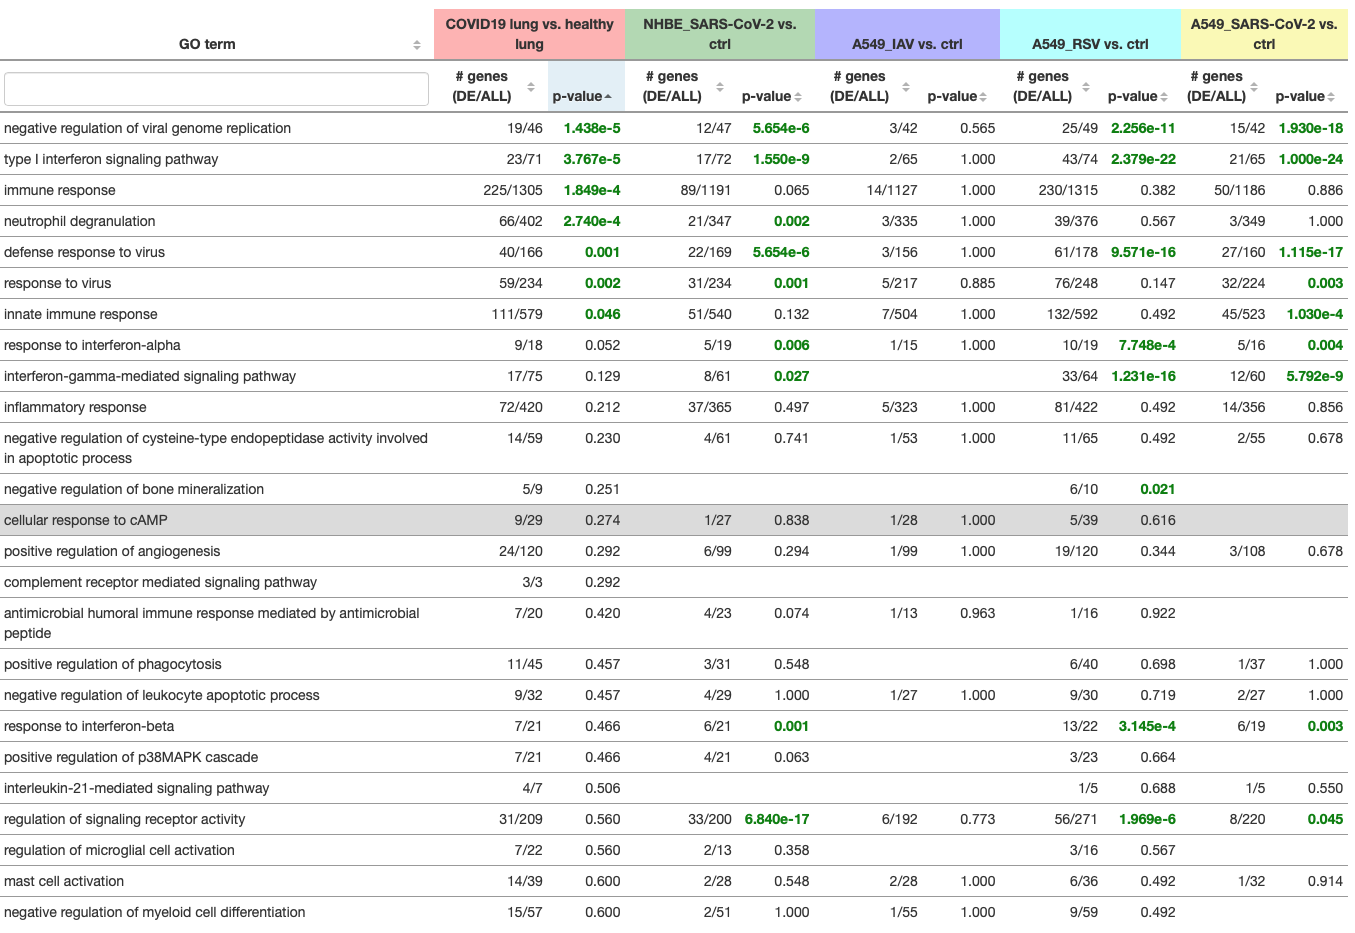
\includegraphics[width=1\linewidth]{Figures/BPs_elim_FDR_all.png}
    \caption{Biological processes (BPs) identified as significant in the five experiments sorted by their significance in the COVID19vsControl. The  columns labelled ``\#genes'' show the number of differentially expressed (DE) genes out of the number of genes associated with the given biological process.  For instance for COVID19vsControl, the most significant BP is negative regulation of viral genome replication: 19 out of the 46 genes known to be involved in this process are differentially expressed and all but one of those are significantly up-regulated.  \label{Supp:BPs}}
        
\end{figure}

\begin{figure}
\centering
	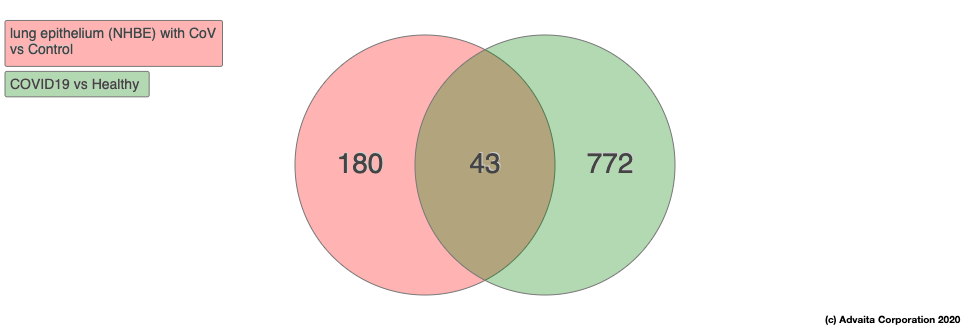
\includegraphics[width=1\linewidth]{Figures/meta_DEGs_patient_NHBE.png}
    \caption{Number of differentially expressed genes in the COVID19vsControl (green) and  NHBECoV2vsControl (red). In spite of the larger number of DE genes in the patient's lung (815), there are only 7 significant biological processes involved (see Figure~\ref{Supp:BPs}) which may indicate a more coordinated, systemic response. In contrast, the changes in the NHBE cells are characterized by fewer DE genes (only 223), but span more uncoordinated biological processes (see Figure~\ref{Supp:BP_orderedby_NHBE}).  }
        \label{Supp:Venngenes} 
\end{figure}


\begin{figure}
\centering
	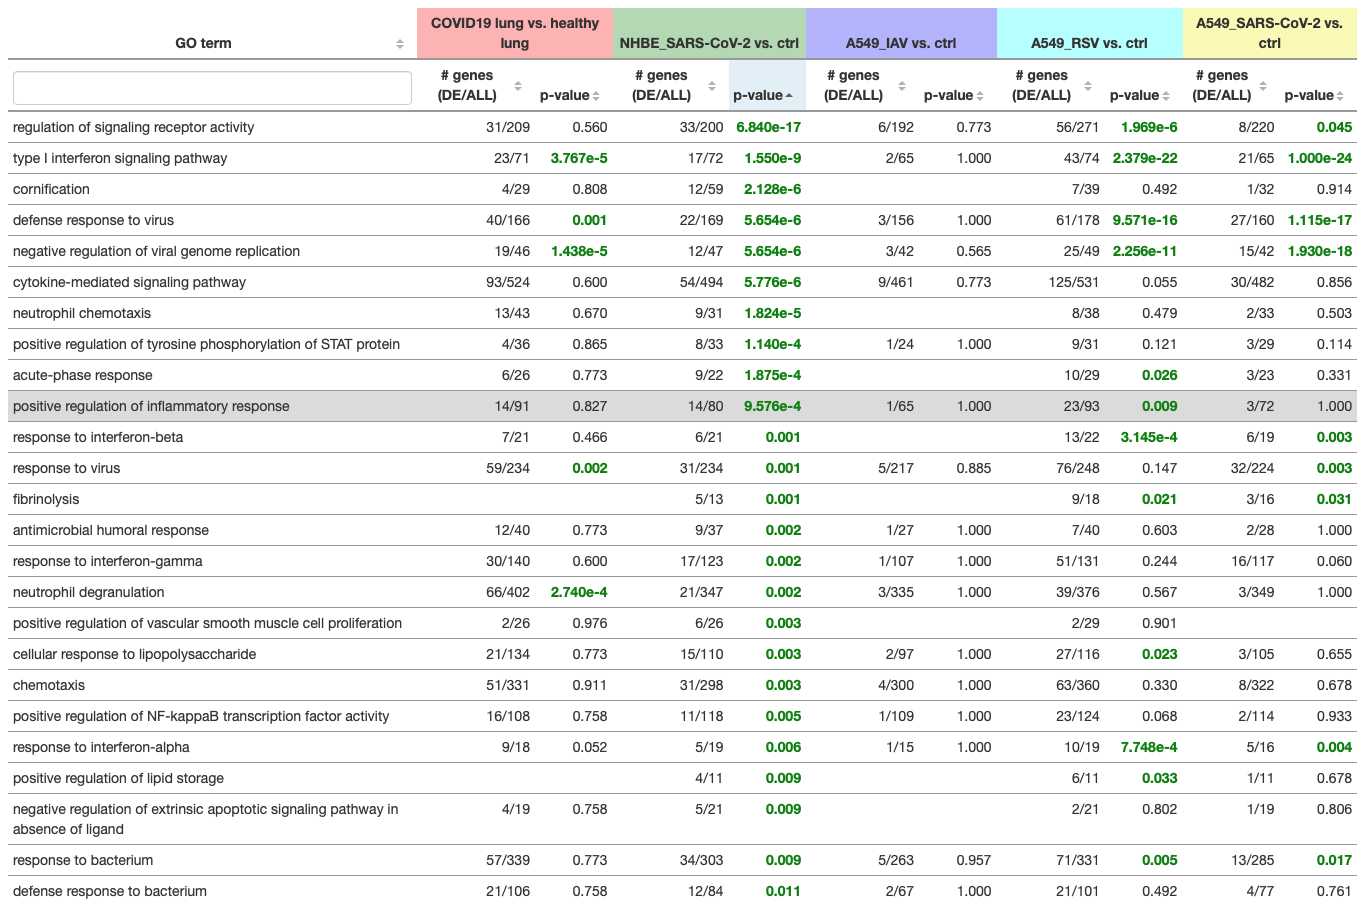
\includegraphics[width=1\linewidth]{Figures/BPs_elim_FDR_all_orderedby_NHBE.png}
    \caption{Biological processes (BPs) identified as significant in the first five experiments sorted by their significance in NHBECoV2vsControl. The  columns labelled ``\#genes'' show the number of differentially expressed (DE) genes out of the number of genes associated with the given biological process. The p-values have been corrected with FDR. }
        \label{Supp:BP_orderedby_NHBE} 
\end{figure}
%in Fig.~\ref{Supp:fig:genes-meta}.

%\textcolor{blue}{add discussion cell lines vs tissue; patient samples; cov2 vs other viruses}

\subsubsection{Putative mechanisms of disease}

We performed an analysis aiming to identify putative mechanisms of  disease. As part of this analysis we identified four genes that were predicted to be activated upstream regulators based on the observed changes in their downstream genes. These were IRF9, STAT2, IFNG, and IFNB1. These suggest two different potential mechanisms. The first appears to be triggered by STAT2 and IRF9, which have 16 common target genes that are also all significantly up-regulated (IFI6, IFIT1, IFIT2, IFIT3, IFITM1, IFITM3, OAS1, OAS3, OAS S32, MX1, MX2, RSAD2, OASL, XAF1, IRF2, and IRF7). This mechanism is also known to be involved in the response to influenza A  (see  influenza A pathway in Fig.~\ref{Supp:influenzaA}). 

\begin{figure}
\centering
%	\includegraphics[width=0.8\linewidth]{influenza_A.png}
	\includegraphics[width=1\linewidth]{Figures/influenza_A.png}
    \caption{The genes found to be differentially expressed in COVID-19 shown on the influenza A pathway. Note the putative mechanism triggered by STAT2 and IRF9 inferred from the SARS-CoV2 data is also present on the response to influenza A pathway shown here (rectangle).   Up-regulated genes are shown in shades of red, down-regulated genes are shown in shades of blue. OAS1, OAS2, OAS3 are grouped together as OAS downstream of IRF9. MX1 and MX2 are grouped together as MXA.  }
        \label{Supp:influenzaA} 
\end{figure}

The second putative mechanism involves interferon beta and gamma, which are targeting 5 common downstream genes: CXCL10, IDO1, DOX58, STAT1, which are up-regulated, and HMOX2 which is down-regulated. Interferon regulatory factors (IRFs) are subdivided into the interferonic IRFs (IRF2-3-7 and 9), the stress responsive IRFs (IRF1 and 5), the hematopoietic IRFs (IRF4 and 8) and morphogenic IRF6. IRF9 is a regulator of type I IFN signaling and is known to interact with STAT2~\cite{horvath1996interactions} and STAT1 to form the heterotrimeric transcription factor complex (ISGF3) that binds to interferon-stimulated response elements (ISREs) to induce the expression of interferon stimulated genes (ISG). During viral infections, ISGs perform two key functions: 1) directly limit viral replication by shutting down protein synthesis and triggering apoptosis; 2) activate key components of the innate and adaptive immune system, including antigen presentation and production of cytokines. The genes triggered by the STAT2 and IRF9 pathway include genes responsible for limiting viral replication (IFI6, IFIT1, IFIT2, IFIT3, IFITM1, IFITM3, OAS1, OAS3, OAS2, MX1, MX2, RSAD2, OASL) and inducers of apoptosis (XAF1, IRF2, IRF7). CXCL10, IDO1, DOX58, and STAT1 are genes associated with lymphocyte recruitment and immune regulation.


Interestingly, STAT2 and IRF9 together are also identified as activated upstream regulators due to 15 downstream targets even in the NHBECoV2vsControl (see Fig.~\ref{Supp:stat2irf9}). However, in the NHBE cells, the interferon activators were replaced by an interleukin based mechanism centered around IL1B, IL6, IL17A, adiponectin (ADIPOQ) and tumor necrosis factor (TNF).

\begin{figure}
\centering
%	\includegraphics[width=0.6\linewidth]{STAT2-IRF9.png}
	\includegraphics[width=1\linewidth]{Figures/STAT2-IRF9.png}
    \caption{ STAT2  and IRF9 are identified as activated upstream regulators due to the 15 genes that are: i) immediately downstream of them, ii) differentially expressed and iii) consistent with their activation.  The colors represent the fold changes measured in COVID19vsControl. STAT2 is shown in gray because was measured to be up-regulated 2.265  fold, but its FDR-corrected p-value was not significant ($p=0.06$).}
        \label{Supp:stat2irf9}
\end{figure}

We also looked at genes that are known to modulate or inhibit the inflammatory response such as IL1RN IL10, and IL13. In the COVID19vsControl, IL1RN was up with a log2 fold change of 6.2 fold (a 78-fold increase, FDR-corrected $p=10^{-6}$),  IL10 was  up 2.8 fold (FDR-corrected $p=0.55$),  while the measurement for IL13 was not available.  In the NHBECoV2vsControl, IL1RN was up only 1.26 fold (FRD-corrected $p=0.035$), while measurements for IL10 and IL13 were not available. 
However, in this contrast, 14 out of 15 DE genes immediately downstream of IL10 and usually inhibited by IL10 were up-regulated which strongly supports the hypothesis that IL10 is inhibited (FDR-corrected $p=5.17\times 10^{-9}$). 

\subsubsection{Impacted pathways}

The significantly impacted  pathways are shown in Fig.~\ref{significant_pathways} and Fig.~\ref{Supp:pathways-meta_Bonferroni} ordered by their significance in COVID19vsControl and NHBECoV2vsControl, respectively. The p-values represent a combination of enrichment and perturbation p-values~\cite{DraghiciPE:2007} subsequently  corrected with FDR.  

\begin{figure}
\centering
%	\includegraphics[width=0.9\linewidth]{significant_pathways_FDR.png}
	\includegraphics[width=1\linewidth]{Figures/significant_pathways_FDR.png}
    \caption{ The signaling pathways found to be significantly impacted in all five experiments ordered by their significance in the COVID19vsControl. The FDR-corrected p-values represent a combination of the p-value due to  enrichment and the p-value due to pathway impact. The column labelled ``\#genes'' shows the number of DE genes  and the total number of genes on each pathway. %\blue{\st{All p-values have been corrected for multiple comparisons wtih FDR}}. 
    }
        \label{significant_pathways}
\end{figure}

\begin{figure}
\centering
	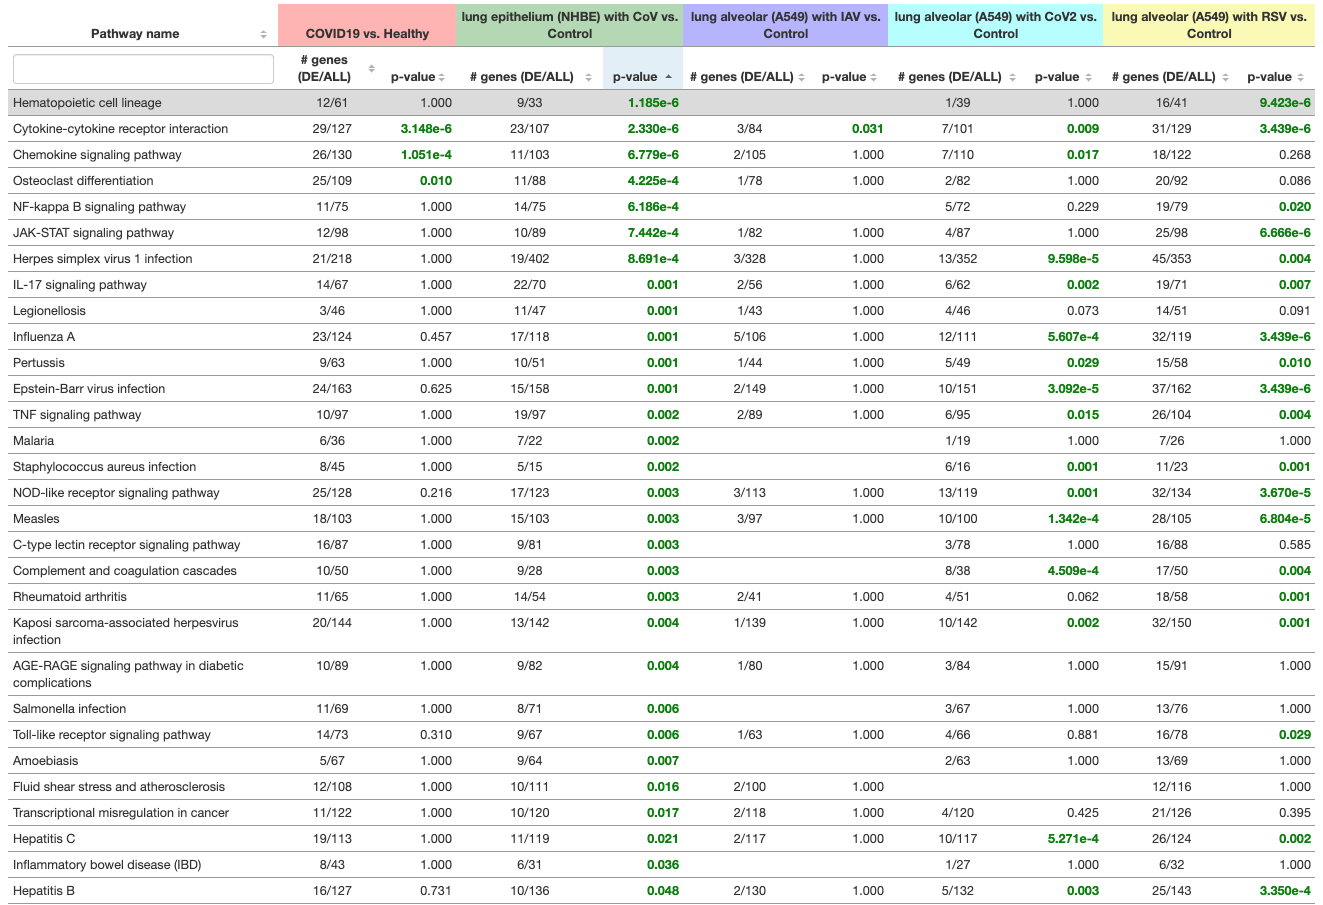
\includegraphics[width=1\linewidth]{Figures/pathways-meta_Bonferroni.png}
    \caption{ The signaling pathways in all 5 experiments, ordered by their significance in NHBECoV2vsControl.  The Bonferroni-corrected p-values represent a combination of the p-value due to  enrichment and the p-value due to pathway impact. The middle column shows the number of DE genes  and the total number of genes on each pathway. 
    The most impacted pathway in NHBE is the hematopoietic pathway which may be linked to the hyper-coagulation phenomena observed in many COVID-19 patients. }
        \label{Supp:pathways-meta_Bonferroni}
\end{figure}

\begin{figure*}
\centering
	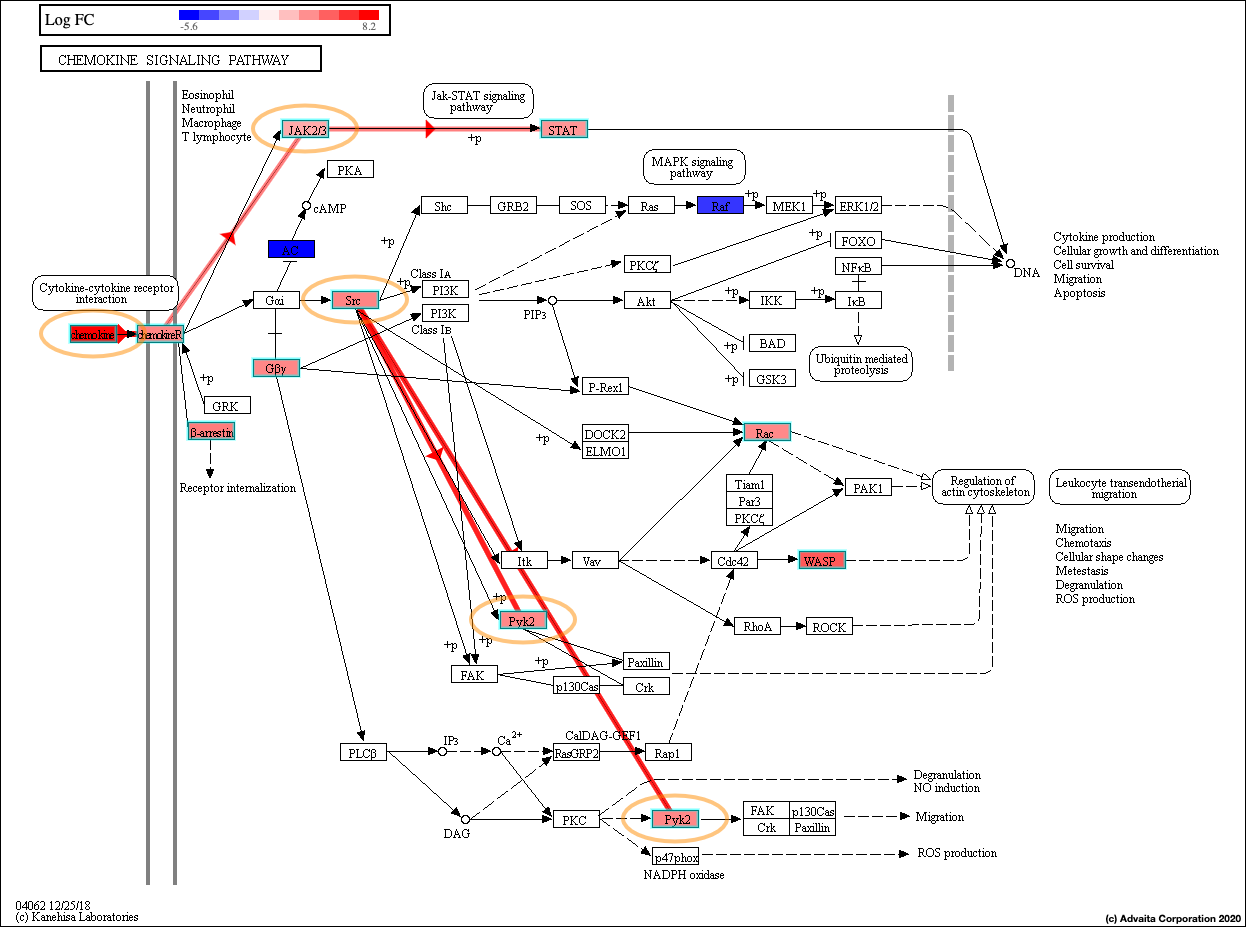
\includegraphics[width=0.9\linewidth]{Figures/Chemokine_signaling_pathway.png}
    \caption{ The chemokine signaling pathway is the second most significantly impacted pathway in COVID19vsControl. The red arrows represent chains of coherent perturbation propagation, i.e. sequence of steps for which the observed expression changes are coherent with the expected changes according to the phenomena described by the pathway. The node labelled ``chemokines'' represents 11 chemokines measured to be up-regulated (CCL2, CCL3, CCL4, CCL7, CCL8, CCL11,  CCL18, CCL19, CXCL10, CXCL11, CXCL16 ). The CCR1 receptor is also up-regulated, as well as  JAK3 and STAT1. The ovals represent drug targets for which FDA-approved drugs already exist. %The drugs targeting genes on this pathway are shown in Fig.~\ref{Supp:drugs_targeting_chemokines}. 
    On this pathway, the impact is due both to the large number of DE genes  (26 out of 130), as well as to the signal propagation as shown by the red arrows. }
        \label{Supp:drugs_on_chemokine_signaling}
\end{figure*}

Fig.~\ref{Supp:cytokine-cytokine_pathway} shows the most impacted pathway, the \emph{Cytokine-cytokine interactions}. 
The gene expression changes on this pathway  show a very large number of pro-inflammatory cytokines and cytokine receptors being up-regulated, while several of the anti-inflammatory genes in the TGF-beta family are down-regulated. This corroborates the GO analysis finding above that there is a very strong positive regulation of inflammatory response. 
\color{black}


Fig.~\ref{Supp:drugs_on_chemokine_signaling} shows the \emph{Chemokine signaling pathway}.  
On this pathway, the impact is due both to the large number of DE genes (26 out of 130), as well as to the clear signal propagation from the chemokines outside the cell (11 chemokines up-regulated), through the chemokine receptor and via the JAK and STAT mechanism. 
Note that the same mechanism is also identified on the Influenza A pathway (see Fig.~\ref{Supp:influenzaA}). 
Fig.~\ref{Supp:chemokine_signaling_mechanism} shows another view of the mechanism involving the genes on this pathway and all their known interactions.

\begin{figure}
\centering
%	\includegraphics[width=0.5\linewidth]{chemokine_signaling_mechanism.png}
	\includegraphics[width=0.8\linewidth]{Figures/chemokine_signaling_mechanism.png}
    \caption{The known interactions involving the genes on the chemokine signaling pathway. }
        \label{Supp:chemokine_signaling_mechanism}
\end{figure}

Another impacted pathway is \emph{Necroptosis}, shown in Fig.~\ref{Supp:necroptosis}. Necroptosis is a programmed form of necrosis, or inflammatory cell death. Conventionally, necrosis is associated with un-programmed cell death resulting from cellular damage or infiltration by pathogens, both of which are probably true in COVID-19-infected lung. Note the IFN - JAK- STAT - PKR  sequence involving up-regulated genes at every step. 

\begin{figure}
\centering
%	\includegraphics[width=0.75\linewidth]{necroptosis.png}
	\includegraphics[width=1\linewidth]{Figures/necroptosis.png}
    \caption{The necroptosis pathway. The genes shown in red are up-regulated while the genes shown in blue are down-regulated.  Note the IFN - JAK- STAT - PKR  sequence involving up-regulated genes at every step. }
        \label{Supp:necroptosis}
\end{figure}

Together, the GO analysis, pathway analysis and the putative mechanisms identified by the analysis above strongly  suggest a hyper-inflammation/cytokine storm.
\color{black} 

\subsubsection{Screening of potential therapeutic approaches: Proposed drugs}  

Once we identified the main regulatory pathways potentially associated with hyper-inflammation, we evaluated \emph{in silico} FDA-approved drugs that could show activity on multiple components of inflammation and consequently could be used for the management of severe COVID-19 cases. We consider the number of DE genes that would be reverted by each drug, as well as calculated a Bonferroni-corrected p-value indicating the suitability of each drug for repurposing in COVID-19 based on two different approaches (see ``Methods'' section). We look for drugs that have both small Benforroni-corrected p-values as well as revert a larger number of DE genes. 
%The top five drugs drug identified by our analysis are shown in Fig.~\ref{top5drugs}. Methylprednisolone (MP) and prednisolone are corticosteroids currently used to modulate the immune response in rheumatoid arthritis.  Diclofenac is a non-steroidal anti-inflammatory drug (NSAID). Tofacitinib is a JAK inhibitor (see the JAK-STAT mechanism identified in  Fig.~\ref{Supp:drugs_on_chemokine_signaling}). Gold sodium thiomalate is an older anti-inflammatory drug, also used in the treatment of rheumatoid arthritis. 
%
%
%\begin{figure}
%\centering
%	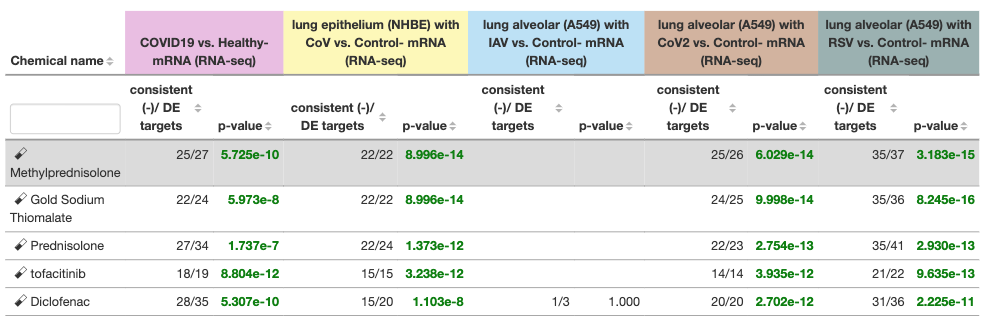
\includegraphics[width=1\linewidth]{Figures/top5drugs.png}
%    \caption{ The top five drugs proposed for repurposing. The table shows both p-values corrected with Bonferroni, as well as the number of DE genes that would be reverted out of the total number of  DE genes immediately downstream  of each drug (annotated as ``consistent (-)/DE targets" in the table).  Methylprednisolone (MP) and prednisolone are corticosteroids currently used to modulate the immune response in rheumatoid arthritis. Gold Sodium Thiomalate is an older drug, not currently in use in the US. Diclofenac is a NSAID and tofacitinib is a JAK inhibitor. The column for A549IAVvsControl is empty because there are no DE genes targeted by these drugs in this contrast.  }
%        \label{top5drugs}
%\end{figure} 


% \textbf{Methylprednisolone} (MP) is the drug that was identified as the most likely to work by inhibiting the inflammatory pathway. This drug targets 27 genes that are found to be DE in COVID19vsControl. Out of these 27 genes, the drug would revert the changes in 25 of them. The drug also had an extremely significant p-value even after a Bonferroni correction which is the most stringent correction available ($p=5.72\times 10^{-10}$). MP also reverted 22 out of 22 genes found to be DE in NHBECoV2vsControl, and 25 out of 26 genes found to be DE in A549CoV2vsControl. 
%Fig.~\ref{common_mechanism}  shows the putative mechanism through which MP acts on the DE genes in COVID19vsControl, and how these genes influence the BPs found to be significantly impacted.

\subsection{Validation on independent data sets}
The initial results obtained on from the data above were subsequently confirmed using additional data, spanning again all  three types of samples: cell lines, tissue cultures, and patient samples.   The additional cell line data include data from Vero E6 cells infected with SARS-CoV-2 vs. controls. Additional tissue cultures include lung organoids infected with SARS-CoV-2 vs. controls. In addition, even though the SARS-CoV-2 virus is primarily thought to infect the lungs with transmission through the respiratory route, it has been suggested that the intestine may present another viral target organ~\cite{Lamers:2020}. For this reason, we also compared the expression profiles of intestine organoids infected with SARS-CoV-2 vs. mock infection in differentiation and expansion media. These data are available in GEO as the GSE153940 (Vero E6 cells)~\cite{Riva:2020}, GSE160435 (lung organoids), and GSE149312 (intestinal organoids)~\cite{Lamers:2020} data sets. 



Finally, twenty nine additional samples from the lung of deceased COVID-19 patients with a high viral load and five controls were included from the Massachusetts General Hospital and Columbia University Irving Medical Center. These are available in GEO as the GSE150316 data set~\cite{desai2020temporal}.

 
Fig.~\ref{Supp:BPs_validation} shows the biological processes common across the five additional independent data sets according to the the classical enrichment analysis. All of these are consistent with a viral response. In particular, the Type I interferon pathway is significant in every single data set analyzed, both initially, as well as in the additional validation data sets. 

The upstream regulators identified in the initial analysis, STAT2 and IRF9, were also found to be significant up-stream regulators in every single validation data set (see Fig.~\ref{Supp:STAT2-IRF9validation}).

Subsequently, we will apply the drug-target analysis on these validation data sets and compare the results obtained with the initial one. 

\begin{figure}
\centering
	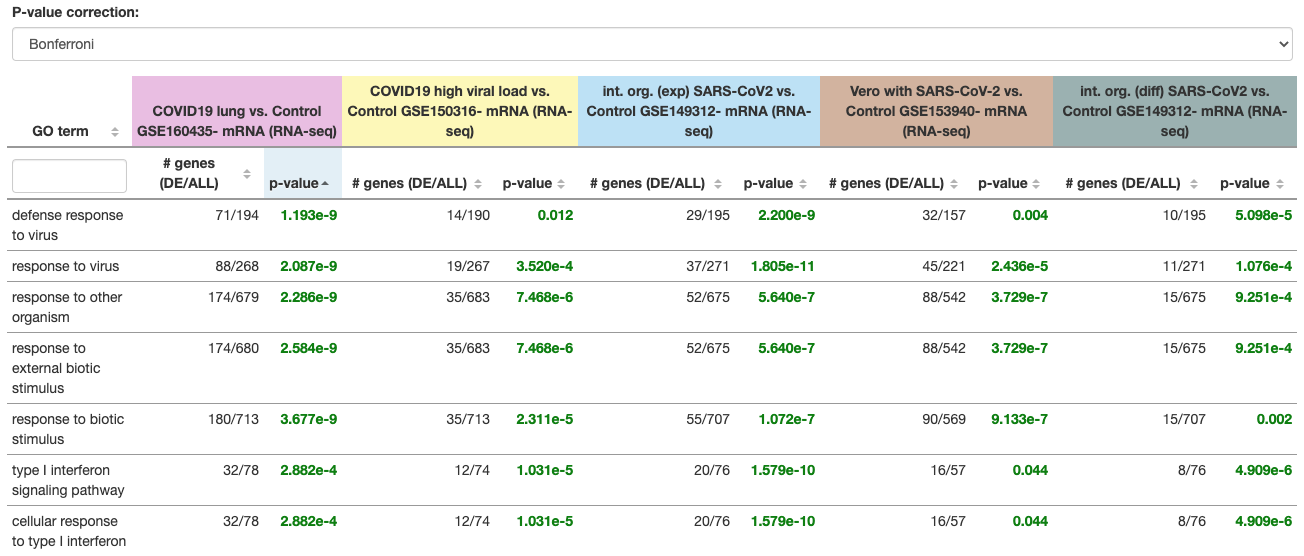
\includegraphics[width=1\linewidth]{Figures/BPs_in_common_(Bonferroni)_in_additional_datasets.png}
    \caption{Biological processes (BPs) identified as significant in the additional independent data sets, as identified by a classical enrichment analysis. The  columns labelled ``\#genes'' show the number of DE genes out of the number of genes associated with the given biological process. The p-values have been corrected with Bonferroni. }
        \label{Supp:BPs_validation} 
\end{figure}

\begin{figure}
\centering
	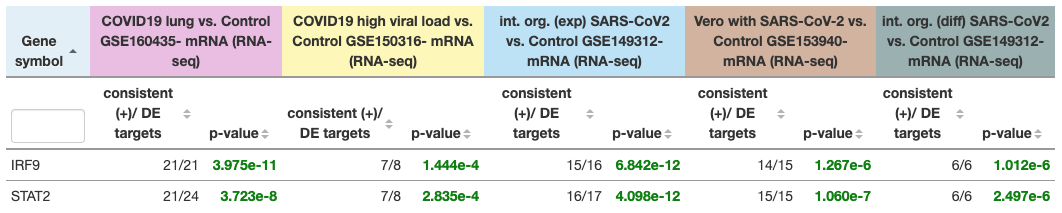
\includegraphics[width=1\linewidth]{Figures/STAT2-IRF9validation.png}
    \caption{The STAT2 and IRF9 were found to be significant upstream regulators in all independent validation data sets. The p-values shown have been corrected with Bonferroni.}
        \label{Supp:STAT2-IRF9validation}
\end{figure}

%Fig.~\ref{Supp:drugs_validation} shows existing FDA-approved drugs identified as suitable candidates for repurposing based on these five additional data sets. These additional and independent data sets span across cell lines, cell cultures and patient data, as detailed above. Note that the top five drugs obtained on these additional data sets are matching perfectly with those shown in Fig.~\ref{top5drugs} even though the data sets analyzed were completely independent.

%\begin{figure}
%\centering
%	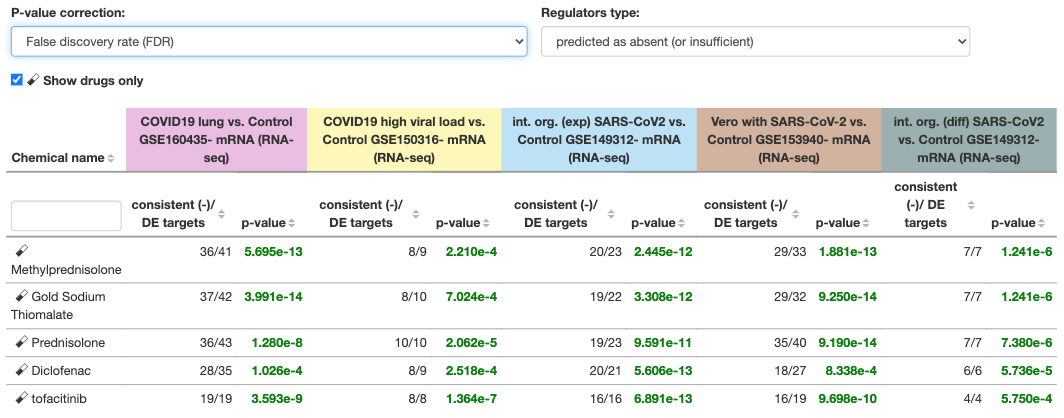
\includegraphics[width=1\linewidth]{Figures/drugs_in_common_(Bonf)_validation.png}
%    \caption{Existing FDA-approved drugs identified as suitable for the treatment of severe COVID-19 cases based on an additional five independent data sets. Note that the top five are identical with those shown in Fig.~\ref{top5drugs} even though the data sets analyzed were completely independent.}
%        \label{Supp:drugs_validation}
%\end{figure}

%
%\subsubsection{In vivo effect of methylprednisolone: Clinical validation.}
%
%
%In an independent study, 213 patients diagnosed with COVID-19 were enrolled. 81 (38\%) received conventional therapy (control group) while 132 patients (62\%) received MP (MP group). The clinical characteristics and treatments received by the patients are shown in Table~\ref{Supp:clinicalcharacteristics} and Table~\ref{additionaltreatment}, respectively. As shown in Table ~\ref{endpoints} thirty day all-cause mortality occurred at a significantly lower rate in the MP group compared to control group ($29.6\%$ vs. $16.6\%, p=0.027$). No statistical difference was detected in the proportion of patients prescribed empiric antibiotics or the time to empiric therapy. Kaplan Meier survival curve for 30-day mortality demonstrated increased probability of survival at 30-days in the MP group as compared to the control group ($p= 0.0204$) (Fig.~\ref{survival}).
%
%\begin{figure}
%\centering
%	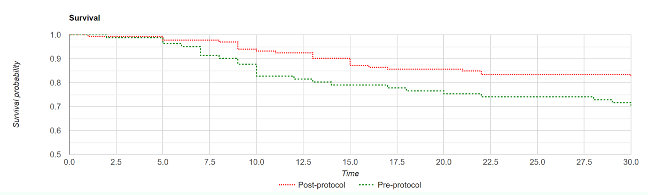
\includegraphics[width=1\linewidth]{Figures/Survival_methylprednisolone.png}
%        \caption{Kaplan Meier survival curve for 30-day mortality demonstrating increased probability of survival at 30-days in the post methylprednisolone cohort as compared to the pre-methylprednisolone cohort (p= 0.0204).  }
%        \label{survival}
%\end{figure}


%When comparing the two groups, those patients treated with a 3-day methylprednisolone protocol spent less time in the hospital (5 vs 8 days) and were less likely to be admitted to the ICU (27\% vs 44\%), being placed on a ventilator (22\% vs 37\%) or dying (14\% vs 26\%).
%
%For a composite end point of preventing ICU admission, need for mechanical ventilator or mortality, the number needed to treat (NNT) to benefit a single patient was only 5 when methylprednisolone was used early in hospitalization. To prevent mortality, the NNT to benefit a single patient was only 8 for all hospitalized patients. This is in contrast to the RECOVERY trial (NCT04323592) for dexamethasone, where NNT was 8 for patients on mechanical ventilation and 25 for patients needed oxygen to prevent mortality.
%\color{black}

%\begin{figure}
%	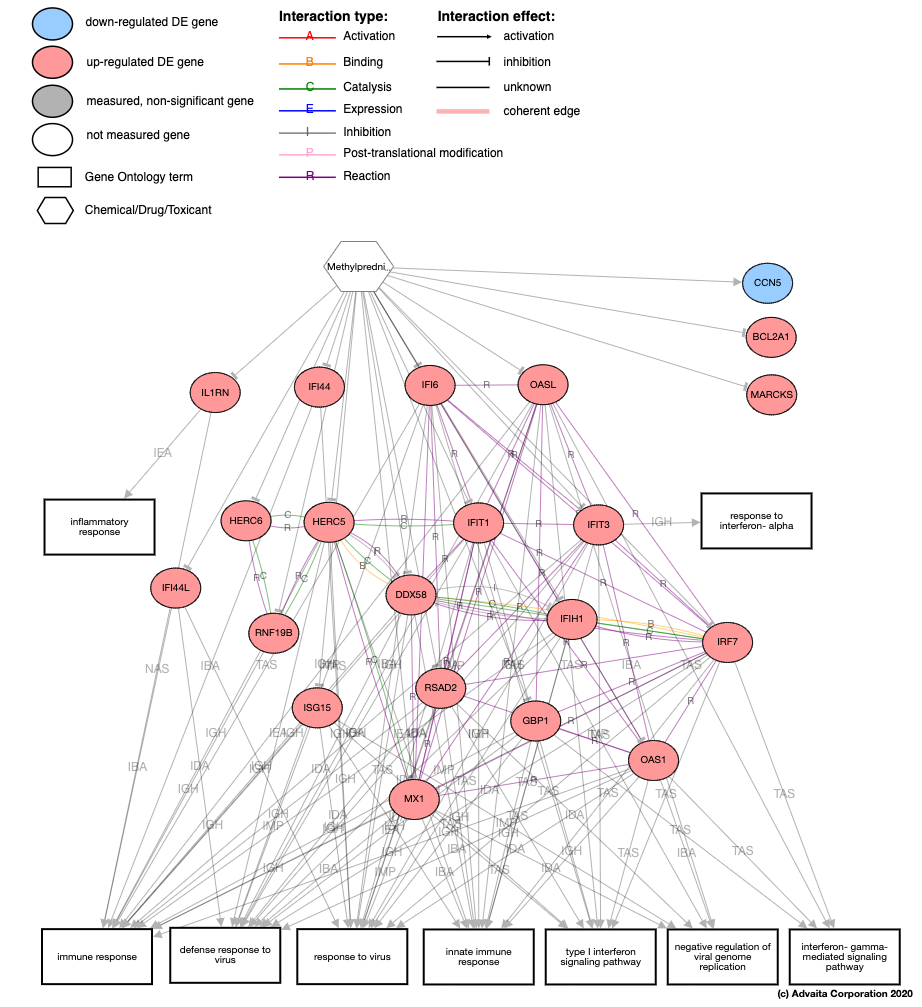
\includegraphics[width=1\linewidth]{Figures/MethylprednisolonetoBPs.png}
%         \caption{The putative mechanism through which MP acts on the genes measured to be DE, and  how these genes influence the  biological processes found to be significantly impacted in  the COVID19vsControl. This figure shows that: i) MP is known to revert the measured changes in all these 21 DE genes; ii) 20 out of these 21 DE genes are up-regulated suggesting a very strong immune response;  ii) many of the DE gene targeted directly by MP are directly involved in the top biological processes identified as significantly perturbed by the disease.} 
%        \label{common_mechanism}
%\end{figure}

%\subsubsection{Other drugs investigated.}
%
%We also looked at other drugs that have already been proposed as repurposing candidates for COVID-19 including: \textbf{chloroquine}, \textbf{hydroxychloroquine}, \textbf{erythromycin},  \textbf{prednisone}, \textbf{dexamethasone},  \textbf{ibuprofen}, \textbf{ritonavir}, \textbf{aspirin}, and \textbf{clopidogrel}. Most or all of these drugs are currently under clinical trials~\cite{sanders2020pharmacologic}. 
%
%\textbf{Chloroquine} was found to revert only 2 out of 4 genes found to be differentially expressed in the COVID19vsControl ($p=1$) and only 3 out of 6 genes found to be differentially expressed in NHBECoV2vsControl only ($p=1$). Furthermore, this drug was not found to be potentially effective in reversing the changes in A549RSVvsControl ($p=1$)  or A549CoV2vsControl ($p=1$). These results suggest that  chloroquine would not be a good potential candidate for repurposing for the goal of modulating the immune response.  
%
%\textbf{Hydroxychloroquine}  did not appear as a good candidate for repurposing in any of the phenotypes and contrasts studied here. 
%Chloroquine and hydroxychloroquine do not target any of the 21 genes that are both severely dysregulated, and also targeted by the proposed drugs. Note that while these drugs do not reverse observed gene expression changes, they may act as anti-virals by potentially inhibiting the viral replication~\cite{sanders2020pharmacologic}.
%
%\textbf{Erythromycin}  targets only three DE genes in COVID19vsControl  and would revert only 2 of those. This yields an insignificant p value (Bonferroni-corrected $p=1$ and FDR-corrected $p=0.75$). 
%
%\textbf{Ibuprofen} was also not found to be a good candidate for use in COVID-19, having the potential to revert only 4 out of 10 DE genes ($p=1$). This suggests a  phenomenon in the class of NSAIDs similar with that observed within the corticosteroids: while one or two specific drugs may be effective, 
%these effects cannot be generalized to the entire class. 
%In other words, not all NSAIDs may be equally helpful in modulating the over-inflammation induced by COVID-19. 
%
%\textbf{Ritonavir} was found to be significant ($p=0.002$) in reverting changes in 8 out of its 10 targets that were measured to be differentially expressed in NHBECoV2vsControl. However, ritonavir was not found to be effective in reversing the gene changes induced in 
%COVID19vsControl.
%
%\textbf{Clopidogrel} targets only one DE gene in COVID19vsControl, one DE gene in A549CoV2vsControl, and no DE gene in NHBECoV2vsControl. These results suggest that this drug is unlikely to be effective in COVID-19 with a p-value of 1 across all experiments. 
% 
% Finally, \textbf{aspirin}  is targeting 44 
% DE genes in COVID19vsControl but  reversing only 22 of them. In NHBECoV2vsControl samples, aspirin was found to target 18 genes and revert 12 on them. In NHBE, aspirin has a raw p-value of 0.028 but after an FDR correction this becomes 0.187. In the COVID19vsControl contrast, even the raw p-value is 0.939 and  becomes 1 after any correction. 
 
%\subsection{Discussion}
%
%In the present study we described an initial characterization of the main pro-inflammatory pathways induced by SARS-Cov-2 infection on human lung epithelial cells and the identification of the most effective therapeutic approach to inhibit this cytokine storm.

%In this study we have identified MP as the most effective, FDA approved, drug that targets critical components of the inflammatory pathway responsible for ARDS.  Furthermore, we demonstrated its efficacy  in a clinical trial in which MP decreased the incidence of mortality in COVID-19 patients. An important finding of this study is that drugs in the same class might not necessarily have similar effects. For instance, MP and prednisolone were predicted to be effective in reverting many of the changes triggered by COVID-19, while other closely-related corticosteroids such as prednisone were not. MP and prednisolone are corticosteroids currently used to modulate the immune response in rheumatoid arthritis. Interestingly, we observed that the putative mechanisms through which these drugs would revert the genes dysregulated in COVID-19 are different (Fig.~\ref{both_mechanisms}). MP for example inhibits STAT1, IFT3 and HERC5 while prednisolone has an impact on IFIT genes such as IFT1, IFIT3, IFI6, and IFI4L.
%
%\begin{figure}
%\centering
%	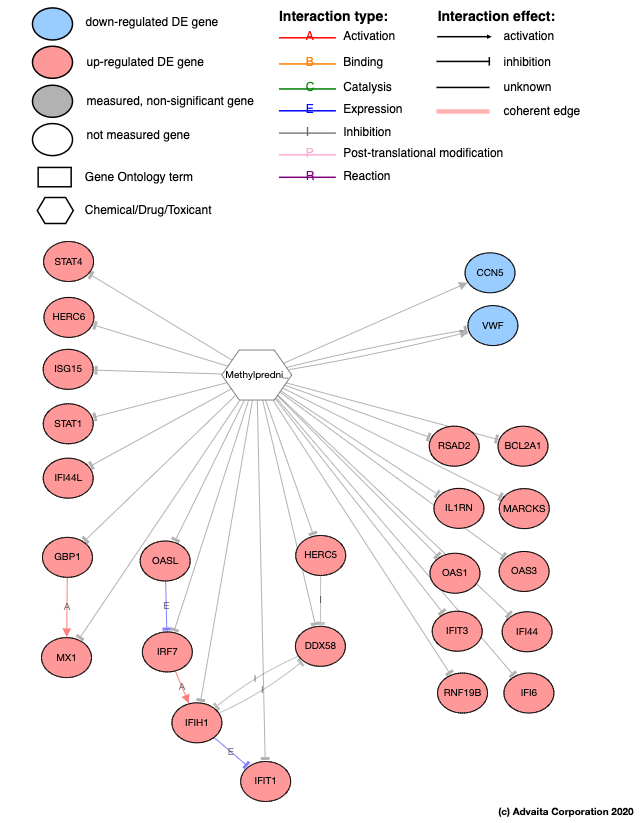
\includegraphics[width=0.8\linewidth]{Figures/Methylprednisolone_mechanism.png}
%        \caption{The putative mechanisms through which methylprednisolone  would revert the  changes triggered by COVID-19  in the lung tissue.}
%        \label{both_mechanisms}
%\end{figure}

%We also looked at other corticosteroids such as prednisone, and hydrocortisone. However, prednisone was found to target only 3 DE genes in the COVID19vsControl and only 2 DE genes in the NHBECoV2vsControl. From those, prednisone would revert only 1 of the 3 DE genes in the COVID19vsControl and 0 out of 2 DE genes in the NHBECoV2vsControl. Both yielded insignificant Bonferroni-corrected p-values ($p=1$) suggesting that prednisone is not expected to be a highly effective treatment. Prednisolone, dexamethasone, and hydrocortisone belong to the same family of corticosteroid anti-inflammatory agents and there is also a structural similarity between them (Fig.~\ref{Supp:steroids}). In spite of this structural similarity, hydrocortisone is known to revert only 8 out of 10 DE genes in the COVID19vsControl (FDR-corrected $p=0.57$) and 5 out of 8 DE genes in the NHBECoV2vsControl (FDR-corrected $p=0.038$, Bonferroni-corrected  $p=1$). Dexamethasone was found to revert 33 out of 69 DE genes in the COVID19vsControl (FDR-corrected $p=1$) and 27 out of 45 DE genes in the NHBECoV2vsControl (FDR-corrected $p=0.002$, Bonferroni-corrected $p=0.066$). Dexamethasone is significant in the NHBECoV2vsControl but not in the COVID19vsControl. Hydrocortisone appears as significant in COVID19vsControl, but only marginally so in the NHBECoV2vsControl.
%


%Such differences between drugs in the same class can be potentially explained in two ways. First, different drugs can be associated with a different number of annotations. For instance, the number of genes that a given drug is known to be targeting can influence its significance. Table~\ref{Supp:drugcoverage}  in Supplementary Materials shows the number of known targets associated with some drugs relevant to COVID-19. Second, there could be genuine differences between the effectiveness of different corticosteroids, potentially due to a different number of genes truly impacted by each drug. The results of these study, based on all annotations available to date, suggest that MP would revert the largest number of the gene perturbed by COVID-19, followed by dexamethasone and, as shown in the outcome of COVID-19 infected patients, have a major impact on their clinical outcome. Prednisone and hydrocortisone revert much fewer known genes and consequently, could have an effect but it is expected to be less effective than the one observed with MP.  Future clinical trials comparing the efficacy of these different corticosteroids are necessary to confirm our findings




%The host inflammatory response in the lungs lead to acute lung injury and ARDS. This constitutes the main rationale for the use of corticosteroids. However, administration of corticosteroids is associated with multiple side effects, such as an increased risk of secondary infection and delayed viral clearance. A recent article in Lancet reports that clinical evidence does not support corticosteroid treatment for COVID-19~\cite{russell2020clinical}. However, this report looks at corticosteroids as an entire class of drugs. A recent retrospective study of 201 patients with COVID-19 in China found that treatment with MP for those who developed ARDS was associated effective in decreasing the risk of death. Among patients with ARDS, treatment with MP decreased the risk of death (HR, 0.38; 95\% CI, 0.20-0.72). In this study, 23 of 50 [46\%] patients with MP treatment died compared to 21 deaths out of  34 patients without MP treatment~\cite{wu2020risk}. Both reports are entirely consistent with our findings: corticosteroids in general are NOT expected to help as a class of drugs, but rather each steroid should be assessed individually.
%
%
%Methylprednisolone has been also the focus on several other recent clinical studies. Wu \emph{et al.} studied the effect of MP  in a cohort of 201 COVID-19 patients, of which 84 developed ARDS~\cite{WuRiskFactorsCOVID:2020}.  They report that ``among patients with ARDS, treatment with MP decreased the risk of death (HR, 0.38; 95\% CI, 0.20-0.72).'' The percentage of people who developed ARDS and eventually died was reduced from  61.8\% (21 of 34) to 46\% (23 of 50).
%
%Salton \emph{et al.}  conducted a multi-center, observational study to explore the association between a prolonged, low-dose of MP and a composite endpoint including the need for ICU referrals, intubation, or death within 28 days (\href{www.clinicaltrials.gov}{www.clinicaltrials.gov}, NCT04323592)~\cite{salton2020prolonged}. They found that in a cohort of 83 patients treated with MP and 90 controls, the treatment with MP significantly lowered the hazard of death (71\%). The composite end point was met by 19 vs. 40 (adjusted hazard ratio (HR) 0.41; 95\% confidence interval (CI): 0.24-0.72). Transfer to ICU and need for invasive MV was necessary in 15 vs. 27 ($p=0.07$) and 14 vs. 26 ($p=0.10$), respectively. By day 28, the MP group had fewer deaths (6 vs. 21, adjusted HR=0.29; 95\% CI: 0.12-0.73) and more days off invasive MV (24.0 +/- 9.0 vs. 17.5 +/- 12.8; $p=0.001$).
%
%A similar multi-center study focus on MP was undertaken in Spain (European Clinical Trials Register: 2020-001934-37). This study involved 85 patients of which 34 were randomized to MP, 22 were assigned to MP by the clinician and 29 constituted the control group. The composite endpoint requirement of non-invasive ventilation, admission to ICU, and death. This study reported that the use of MP was associated with a reduced risk of the composite endpoint  (RR 0.55 95\% CI 0.33-0.91) (\href{https://www.medrxiv.org/content/10.1101/2020.06.17.20133579v1}{https://www.medrxiv.org/content/10.1101/2020.06.17.20133579v1}).

%Finally, preliminary results from a large randomized study undertaken in the UK (NCT04381936) show that dexamethasone is also able to significantly reduce the number of deaths. In this study the steroid group included 2,100 participants and was compared with the standard of care group including 4,300 participants. Unfortunately, this study placed dexamethasone in the same arm with MP (MP to be administered to pregnant women instead of dexamethasone), so this study will not be able to elucidate whether MP and dexamethasone have any differences in efficacy. However, the results of the clinical study presented here suggest that MP has a lower NNT than dexamethasone. The potential higher efficacy of MP needs to be confirmed in larger cohorts. However, in a recent meta-analysis of randomized studies investigating prolonged corticosteroid treatment in non-viral ARDS, methylprednisolone treatment achieved a reduction in duration of mechanical ventilation and mortality superior to that of dexamethasone or hydrocortisone~\cite{meduri2020pharmacological}.

%We also looked at other drugs that have already been proposed as repurposing candidates for COVID-19 including: chloroquine, hydroxychloroquine, erythromycin, prednisone, ibuprofen, ritonavir, aspirin, and clopidogrel. None of these was predicted to be effective in reverting SARS-CoV2 gene expression changes (see Supplementary Materials).
 
%In summary, we describe the inflammatory pathways associated with the cytokine storm found in COVID-19 patients and describe the characterization of the potential effective therapeutic approaches that, by targeting these pathways could effectible reduce the hyper-inflammatory response responsible for the development of ARDS, a main cause of mortality in COVID-19 patients.  Clinical results confirmed the efficacy of the \emph{in silico} prediction that indicated MP could improve outcomes in severe COVID-19. 

\subsection{Methods}


\subsubsection{Gene Ontology (GO) analysis method}  

For each GO term~\cite{ashburner2002ontologies, gene2004gene}, the number of differentially expressed (DE) genes annotated to the term is compared to the number of DE genes expected just by chance. We used  an over-representation approach to compute the statistical significance of observing at least the given number of DE genes, as proposed by~\cite{Tavazoie:1999}. The uncorrected p-value is computed using the hypergeometric distribution, as previously described~\cite{DraghiciOE2:2003,DraghiciBook:2011}, and corrected with FDR and Bonferroni.

The classical method used above considers all GO terms to be independent. However, given the nature of gene ontology, considering the genes multiple times introduces errors~\cite{Rhee:2008,DraghiciBook:2011}. Due to the ``true path rule'', all  genes annotated to a GO term are also annotated to all its ancestors when traversing ``is a'' relationships. Because of this, the same genes are counted in the enrichment of every term above the one they are directly annotated with.  We used an approach inspired by  the \textit{elim} and \emph{weight} pruning methods as originally proposed by Alexa \textit{et al.}~\cite{Alexa:2006}. The algorithm constructs a custom cut through the GO hierarchy by starting with the most specific nodes and calculating their uncorrected p-value with all genes assigned directly to each such node. If a node is significant, it is reported as such. If the node is not significant, the genes associated to the given node are propagated to its direct ancestors and a uncorrected p-value is calculated for each of those. 

\subsubsection{Pathway analysis method}  

The pathways analysis was performed using the Impact Analysis method~\cite{DraghiciPE:2007, tarca2009novel, khatri2007}. The impact analysis uses two types of evidence: i) the over-representation of differentially expressed (DE) genes in a given pathway and ii) the perturbation of that pathway computed by propagating the measured expression changes across the pathway topology. These aspects are captured by two independent probability values, $pORA$ and $pAcc$, that are then combined in a unique pathway-specific uncorrected p-value. The underlying pathway topologies, comprised of genes and their directional interactions, are obtained from the KEGG database~\cite{ogata1999kegg, kanehisa2010kegg, kanehisa2012kegg,  kanehisa2014data}.

The first probability, $pORA$, expresses the probability of observing the number of DE genes in a given pathway that is greater than or equal to the number observed, by random chance~\cite{DraghiciOE2:2003,DraghiciBook:2011}. Let us consider there are $N$ genes measured in the experiment, with $K$ of these on the given pathway. Based on the user-defined a priori selection of DE genes, $n$ out of $N$ genes were found to be differentially expressed. The probability of observing exactly $k$ differentially expressed genes on the given pathway is computed based on the hypergeometric distribution.

Because the hypergeometric distribution is discrete, the probability of observing fewer than $k$ or more genes on the given pathway just by chance is defined as 1 minus  the hypergeometric cumulative density function evaluated at $k-1$.

The second probability, $pAcc$, is calculated based on the amount of total accumulation measured in each pathway. A perturbation factor is computed for each gene on the pathway using:

\begin{equation}
\label{eqn:PF}
PF(g) = \alpha(g) \cdot \Delta E(g) + \sum_{u \in US_g} \beta_{ug}\frac{PF(u)}{N_{ds}(u)}
\end{equation}


In Equation~\ref{eqn:PF}, $PF(g)$ is the perturbation factor for gene $g$, the term $\Delta E(g)$ represents the observed fold change of gene $g$, and $\alpha(g)$ is an a priori weight that can be used to incorporate information about the type of gene or its significance~\cite{voichita2012incorporating}. In this analysis, all gene were treated equally (all $\alpha(g)=1$). The last term is the sum of the perturbation factors of all genes $u$, directly upstream of the target gene $g$, normalized by the number of downstream genes of each such gene $N_{ds}(u)$. The value of $\beta_{ug}$ quantifies the strength of the interaction between genes $g$ and $u$. The sign of $\beta$ represents the type of interaction: positive for activation-like signals, and negative for inhibition-like signals. Subsequently, iPathwayGuide calculates the accumulation at the level of each gene, $Acc(g)$, as the difference between the perturbation factor $PF(g)$ and the observed fold change:

\begin{equation}
Acc(g) = PF(g) - \Delta E(g)
\label{eqn:acc}
\end{equation}

All perturbation accumulations are computed at the same time by solving the system of linear equations resulting from combining Equation~\ref{eqn:PF} for all genes on a given pathway. Once all gene perturbation accumulations are computed, iPathwayGuide computes the total accumulation of the pathway as the sum of all absolute accumulations of the genes in a given pathway. The significance of obtaining a total accumulation ($pAcc$) at least as large as observed, just by chance, is assessed through bootstrap analysis.

The two types of evidence, $pORA$ and $pAcc$, are combined into an overall pathway score by calculating an uncorrected p-value using Fisher's method. This p-value is then corrected for multiple comparisons using false discovery rate (FDR)~\cite{Benjamini:1995,  Benjamini:2001} and Bonferroni~\cite{Bonferroni:1935} corrections. 

The underlying pathway topologies, comprised of genes and their directional interactions, are obtained from the KEGG database~\cite{ogata1999kegg, kanehisa2010kegg, kanehisa2012kegg,  kanehisa2014data}.

\subsubsection{Putative mechanism inference} 

The impact analysis  allows the computation of the perturbation at the level of every gene on every pathway. Putative mechanisms are identified as sequences of pathway signals for which the measured gene expression changes are consistent with the sequence of events described by the pathway. An example would be the chemokine-chemokine receptor-JAK-STAT sequence identified on the Chemokine Signaling Pathway  in Fig.~\ref{Supp:drugs_on_chemokine_signaling}. This approach is able to identify candidates for potentially active mechanisms on existing pathways and has also been shown to have an increased accuracy~\cite{nguyen2019identifying}. %In order to 


\subsubsection{The prediction of upstream Chemicals, Drugs, Toxicants (CDTs)}  

Our approach is based on two types of information: i) the enrichment of DE genes from the experiment and ii) a network of interactions from the Advaita Knowledge Base (AKB v1910). The network is a directed graph in which the source node represents either a chemical substance or compound, a drug, or a toxicant (CDT). We focused our work on FDA-approved drugs that could be repurposed. The edges represent known effects that these CDTs have on various genes. A signed edge in this graph consists of a source CDT ($u$), a target gene, and a sign to indicate the type of effect: activation ($+1$) or inhibition ($-1$). 
The variable $u$ here stands for a CTD but its role is similar to the role of the upstream gene as used in Equation~\ref{eqn:PF} in the impact analysis. In both cases, the analysis is performed on a graph in which ``u'' is the immediately upstream node. In the impact analysis, the upstream node was  a gene whereas here, the upstream node will represent a CTD.

The analysis considers the hypothesis that  the upstream chemical, drug or toxicant is absent (or insufficient) in the condition studied. In essence, a drug for which this hypothesis is supported by a significant amount of evidence will be a very strong candidate for repurposing because such drug will effectively reverse many of the gene expression changes observed in the given disease. 


The analysis divides the set of all the genes from the AKB into several subsets based on the measurements in the experiment and the definitions shown in Fig.~\ref{TwoHypotheses} and Fig. ~\ref{MeasuredGenes}. 
%Let the sign of a measured DE gene be the sign of the log fold change value: ($+$) for up-regulated genes and ($-$) for down-regulated genes. 
A gene is a target gene if it corresponds to a node in the network that has at least one incoming edge. We define a consistent gene as a target DE gene such that the sign of the gene is consistent both with the type of the signal and with the hypothesis considered. 
%Formally, by definition, a target DE gene g is consistent with the testing hypothesis if and only if an incoming edge $e$ exists such that $sign(g) \neq sign(e)$. 
This case captures the situation in which the CDT is absent (or insufficient), the signal is inhibition and the target DE gene is up-regulated, or the signal is activation and the target DE gene is down-regulated (see Fig.~\ref{TwoHypotheses}).

\begin{figure}
\centering
	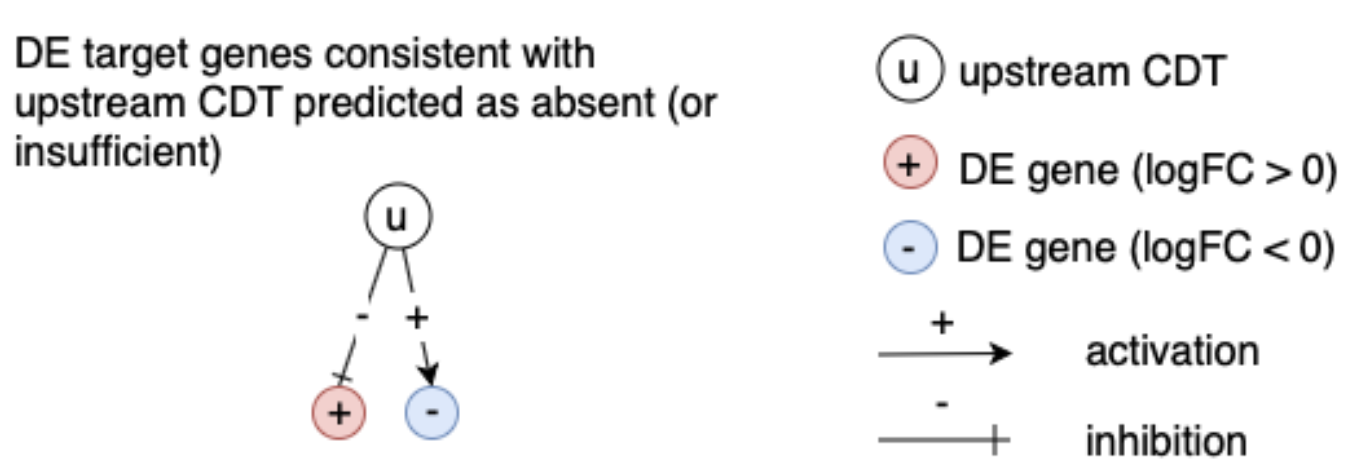
\includegraphics[width=0.6\linewidth]{Figures/TwoHypotheses.png}
        \caption{A candidate for repurposing would revert the changes of the  observed DE genes. This potential drug \emph{u} would repress the  gene which is up-regulated by the disease (red circle) and would activate the one that is repressed (blue circle). }
        \label{TwoHypotheses}
\end{figure}

\begin{figure}
	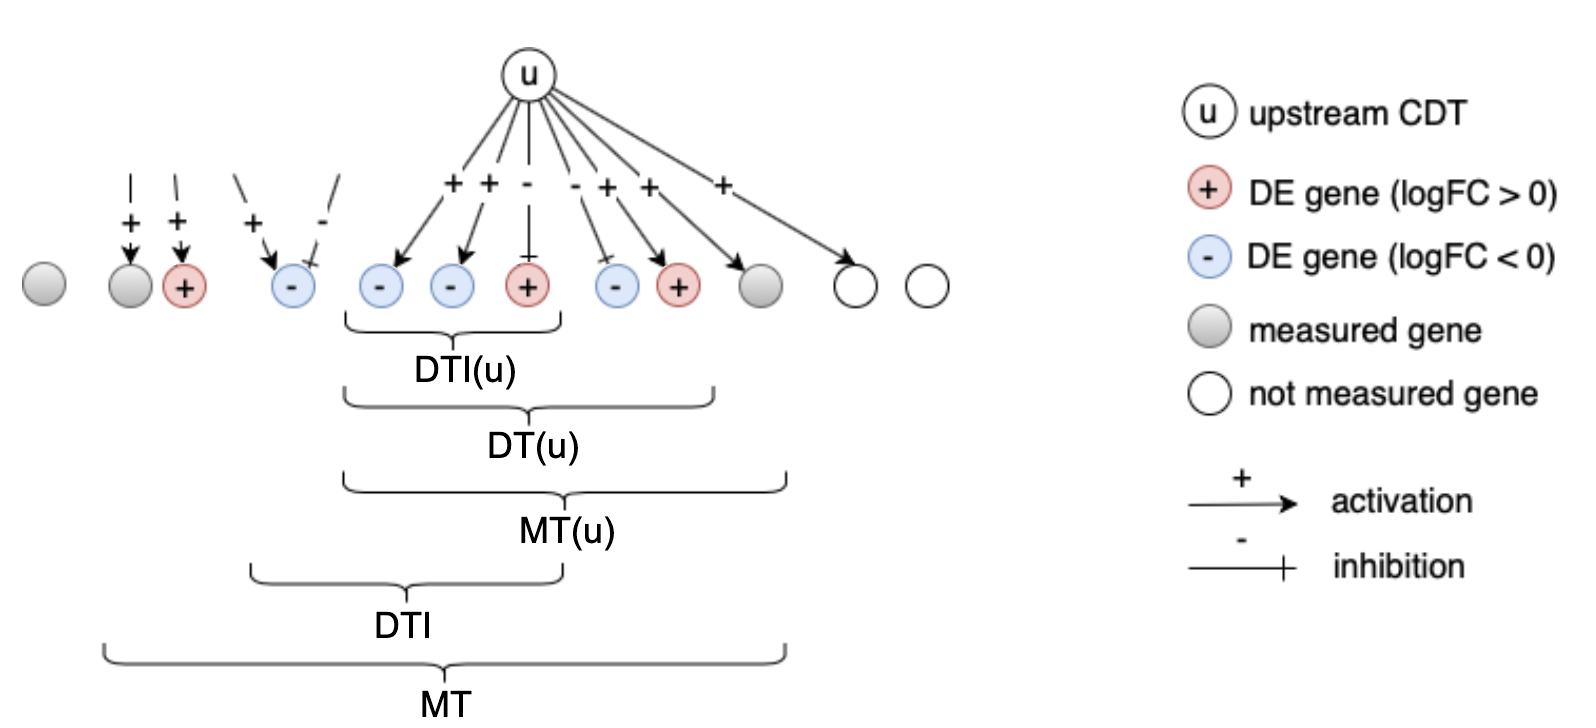
\includegraphics[width=0.9\linewidth]{Figures/MeasuredGenes.png}
        \caption{The set of all genes includes the set of measured genes that are also targets in the network, or Measured Targets (MT). We define the subset of ``DE Targets consistent with the hypothesis that the CDTs are  insufficient'', DTI. For a selected upstream CDT \emph{u}, we have the set of ``Measured Targets of u'' MT(u), ``Differentially expressed Targets downstream of u'' DT(u), and the set of ``DE targets consistent with the hypothesis that u is insufficient'' DTI(u).}
        \label{MeasuredGenes}
\end{figure}

%\textit{Z-score}\\
\newpage

For the research hypothesis considered, the analysis computes a z-score, $z(u)$, for each CDT $u$, by iterating over the genes that are differentially expressed and immediately downstream of $u$, $DT(u)$: 
%the analysis computes a Z-score for each upstream regulator $z(u)$ by iterating over the genes in DT(u) and their incoming edges $in(g)$. 


%\begin{equation}
%\label{eq:zscore}
%z(u)=\frac{\sum\limits_{g \in DT(u)} \sum\limits_{e \in in(g)} sign(e) \times sign(g)}{\sqrt{\sum\limits_{g \in DT(u)} |in(g)}|}
%\end{equation}

\begin{equation}
\label{eq:zscore}
z(u)=\frac{\sum\limits_{g \in DT(u)} sign(e(u,g)) \times sign(g)}{\sqrt{|DT(u)|}}
\end{equation}

where $sign(g)$ is the sign of the DE gene $g$ (1 for up-regulated and -1 for down-regulated), $e(u,g)$ represents an edge from $u$ to $g$,  $sign(e(u,g))$ reflects its type of interaction ($1$ for activation and $-1$ for inhibition), and $|DT(u)|$ represents the number of genes that are differentially expressed and immediately downstream of $u$. 


Under the null hypothesis, the sign of an edge, $sign(e_i)$, and the sign of a gene, $sign(g_i)$, are independent and identically distributed random variables that have either values $-1$ or $1$.  Let $X_i = sign(e_i) \times sign(g_i)$ denote the product of these two variables. Therefore, $X_i$ is also a random variable taking values from $\{-1,1\}$, with the expected value $E[X_i] = \mu = 0$, variance $Var[X_i] = \sigma^2 = 1$. Considering an upstream CDT with $n$ downstream genes ($n = |DT(u)|$), the  average of $n$ samples of $X_i, i \in \{1,...,n\}$ is $\overline{X}_n$.  According to the central limit theorem, the variables $\sqrt{n}(\overline{X}_n - \mu)$ converge  to a normal distribution $N(0,1)$ for large values of $n$. With $\mu = 0$, those variables can be written as:

\begin{equation}
%\label{eq:VariableXn}
\sqrt{n} \cdot \overline{X}_n = \frac{n \cdot \overline{X}_n} {\sqrt{n}} = \frac{n \cdot \frac{\sum_{i=1}^n X_i}{n}}{\sqrt{n}} = \frac{\sum_{i=1}^n X_i}{\sqrt{n}}
\end{equation}

The numerator is actually the sum of all $n$ samples $X_i$, $\sum{X_i}$, which is also the numerator of equation \ref{eq:zscore}. 
%Moreover, the denominator of equation \ref{eq:zscore}, $\sum\limits_{g \in DT(u)} |in(g)| $, is indeed $n$, the number samples. 
Moreover, we have $n = |DT(u)|$.
Hence, we can conclude that the variable $z(u)$ follows a standard normal distribution, $N(0,1)$. Therefore, we can compute the p-value corresponding to the z-score $P_z$ as the one-tail area under the probability density function for normal distribution.

A good candidate for repurposing would revert many of changes observed. This is equivalent  with the research hypothesis that considers the condition is due to a given CDT that is present in insufficient amounts.
We use $P_{abs}$ and $P_z$ to predict upstream CDTs that would revert the measured changes. 
For each upstream CDT $u$, the number of consistent DE genes downstream of $u$, $DTI(u)$, is compared to the number of measured target genes expected to be both consistent and DE just by chance. The uncorrected p-value $P_{abs}$ is computed using the hypergeometric distribution~\cite{DraghiciOT:2003, DraghiciBook:2011}. The analysis combines $P_{abs}$ and $P_z$, using  Fisher's method~\cite{fisher1925statistical}. 

%
%\textbf{Clinical Validation.} 
%We evaluated the MP protocol with a single pretest, single post-test quasi-experiment from March 12-March 27, 2020 at a 5 hospital health system in Michigan. Patients were compared before and after implementation of the MP protocol on March 20th. The clinical characteristics of the patients are shown in Table~\ref{Supp:clinicalcharacteristics}. 
%The primary endpoint was 30 day all-cause mortality.  
%
%
%
%\begin{table}
%\caption{Baseline Demographics and Clinical Characteristics of Study Patients }
%\begin{center}
%\begin{tabular}{p{6.5cm} cccc}
%\hline
%\textbf{Characteristics}  	&\makecell{\textbf{Total} \\ \textbf{(n=213)} }	& \makecell{\textbf{Pre-Protocol} \\ \textbf{(n=81)}} &	\makecell{\textbf{Post-Protocol}\\ \textbf{(n=132)}}	& \textbf{p-value}\\
%\hline
%\multicolumn{5}{l}{\textbf{Demographics}}\\
%\hline
%Age - median (IQR) - years &	62 (51-62)	 & 64 (51.5-3.5)	&61 (51-72)	& 0.400 \\
%Male sex - no. (\%)	&109 (51.2)&	41 (50.6)	&68 (51.5)&	0.899\\
%\multicolumn{5}{l}{Race}\\
%\tab Black - no. (\%)	&	155 (72.8)	&	50 (61.7)	&	105 (79.5)&	0.004\\
%\tab White - no. (\%) 	&	29 (13.6)	&18 (22.2)		&	11 (8.33)	&	0.005\\
%Body mass index (IQR) - median (IQR) - kg/m$^{2}$	&32 (27.3-38.7)	&	30 (25-39)		&	33.2 (28.9-38.5)	&	0.007\\
%\hline
%\multicolumn{5}{l}{\textbf{Comorbidities } - no. (\%)}\\
%\hline
%Asthma &	33 (15.5)&	16 (19.8)	&17 (12.9)	&0.180\\
%Chronic kidney disease  &	98 (46)	&41 (51.9)	&57 (43.5)&	0.240\\
%Chronic obstructive pulmonary disease  &	27 (12.7)	&15 (18.5)	&12 (9.1)	&0.045\\
%Congestive heart failure &	26 (12.2)	&10 (12.5)	&16 (12.2)&	0.951\\
%Coronary artery disease &	38 (17.8)	&18 (22.2)	&20 (15.2)&	0.192\\
%Diabetes	&105 (49.3)&	37 (45.7)	&68 (51.5)	&0.411\\
%Hypertension& 	158 (74.2)	&62 (76.5)	&96 (72.7)	&0.925\\
%Malignancy  	&24 (11.3)	&11 (13.6)	&13 (9.9)	&0.405\\
%Smoking history  	&88 (41.3)&	40 (49.4)	&48 (36.4)&	0.0615\\
%\hline
%\multicolumn{5}{l}{\textbf{Presenting Symptoms}}\\
%\hline
%Cough - no. (\%)	&158 (74.2)	&62 (76.5)&	96 (72.7)	&0.536\\
%Fever - no. (\%)	&150 (70.4)&	57 (70.4)	&93 (70.5)	&0.989\\
%Myalgia - no. (\%)	&85 (39.9)&	32 (39.5)&	53 (40.2)	&0.926\\
%Shortness of breath - no. (\%)	&148 (69.5)&	50 (61.7)	&98 (74.2)	&0.054\\
%Duration of symptoms - median (IQR) - days&	5 (3-7)&	5 (2-7)&	6 (3-7)	&0.107\\
%\hline
%\multicolumn{5}{l}{\textbf{Severity of illness in emergency department (ED)}}\\
%\hline
%qSOFA -- median (IQR)	&1 (0-1)	&1 (0-1)	&1 (0-1)	&0.850\\
%NEWS -- median (IQR)&	7 (4-10)	&7 (4-10)	&7 (4-9)	&0.668\\
%Requiring mechanical ventilation in ED -- no. (\%)	&22 (10.3)&	10 (12.3)&	12 (9.1)	&0.448\\
%Direct admission to ICU -- no. (\%)	&26 (12.2)&	11 (13.6)	&15 (11.4)&	0.631\\
%\hline
%\multicolumn{5}{L{17cm}}{\small *IQR denotes Interquartile range, NEWS denotes National Early Warning Score, qSOFA denotes quick Sequential Organ Failure Assessment (qSOFA), ED denotes Emergency Department, ICU denotes intensive care unit} \\
%\end{tabular}
%\end{center}
%\label{Supp:clinicalcharacteristics}
%\end{table}%
%
%\textbf{The methylprednisolone protocol.}  
%Patients with PCR confirmed COVID-19 who required 4 liters or more of oxygen per minute on admission, or who had escalating oxygen requirements from baseline, were recommended to receive IV methylprednisolone 0.5 to 1 mg/kg/day in 2 divided doses for 3 days. Patients who required ICU admission were eligible to extend the IV methylprednisolone course to a maximum of 7 days at the discretion of the medical team. Institutional guidelines also recommended hydroxychloroquine 400 mg twice daily for 2 doses on day 1, followed by 200 mg twice daily on days 2--5.
%
%\textbf{Statistical Analysis of clinical data.} Survival analysis was performed using the Kaplan-Meier method and log-rank test. More details about the statistical analysis and characteristics of the patient population are included in the Supplementary Materials.
%

%\subsection{Conclusion}
%This paper presents an approach for drug repurposing based on identifying drugs that could revert
%gene expression changes associated with most perturbed biological processes and pathways. Results from a clinical study undertaken in a cohort of 213 patients in a multi-center hospital system confirmed the efficacy of the \emph{in silico} prediction that indicated MP could improve outcomes in severe COVID-19. 
%This prediction is also supported by the results of independent clinical studies with the same drug undertaken in Italy (173 patients) and Spain (85 patients). The drug repurposing approach described here, as well as the drugs identified, might be important for any future pandemic involving hyper-inflammation.









\clearpage

\section{Conclusion}
\label{chap:Conclusion}

\subsection{PURE}

In the doctoral dissertation, we present the the approaches that identify the causal drugs/chemicals that have impact on gene expression profiles. On one hand, it can be used in pin-point the abundance harmful substances in the subject's system, and hence helps doctors to find a suitable treatment. On the other hand, these methods are extremely useful for researchers and doctors in repurpose drugs for alternative application, especially for new viruses or diseases such as COVID-19. These two applications are realized by two following studies.

In Chapter 2, we introduce a method, PURE, that tested two hypotheses that a CDT is responsible for the gene expression changes, which in turn causes the observed phenotype: the level of the CDT in the subject's system is higher than usual or the level of the CDT in the subject's system is lower than usual. The first hypothesis is a crucial ability for the correct identification of the presence of chemicals, drugs or toxicants in studied phenotypes.  With the second hypothesis, PURE can identify the CDT that can revert disease-induced gene expression changes. This capability is expected to be useful in any drug repurposing application. 
The proposed approach was validated using 16 gene expression data sets from 3 different species where the true CDTs that caused the phenotypes were known. We also compared PURE to 5 other methods including a commercial tool, IPA. PURE outperformed all other methods in terms of the rank of the true CDT and the number of false positives in the list of significant CDTs.

In Chapter 3, we used another approach to identify upstream CDTs coupled with a pathway analysis, to investigate an alternative treatment for severe symptoms related to hyper-inflammation of COVID-19 patients~\cite{DraghiciCOVID:2021}. The gene ontology analysis and pathway analysis methods on studied datasets have both confirmed that the cytokine storm is found in COVID-19 samples in this study. Applying the approach to identify upstream regulators would derive a list of proposed drugs that potentially reverse the DE genes and therefore, suppress the cytokine storms. We validated the results with another gene expression dataset. Subsequently, we will validate the proposed drug with an independent clinical trial.
\clearpage

% Compile Appendix A
\phantomsection
% Create appendix with unnumbered section
\section*{APPENDIX A}

% Add appendix to toc at section level
\addcontentsline{toc}{section}{Appendix A}
\appendix{Stuff and Things}
\label{appendix:stuffAndThings}

My Appendix A...

\clearpage

% Compile Appendix B
\phantomsection
% Create appendix with unnumbered section
\section*{APPENDIX B}

% Add appendix to toc at section level
\addcontentsline{toc}{section}{Appendix B}
\appendix{More Stuff and Things}
\label{appendix:moreStuffAndThings}

My Appendix B...

\clearpage

% ...

% Compile Appendix Z
\phantomsection
% Create appendix with unnumbered section
\section*{APPENDIX Z}

% Add appendix to toc at section level
\addcontentsline{toc}{section}{Appendix Z}
\appendix{More Stuff and Things, Again}
\label{appendix:moreStuffAndThingsAgain}

My Appendix Z...

\clearpage

% Compile bibliography
\phantomsection
%% Create references using the unnumbered section formatting
\section*{REFERENCES}

% Add table of contents marker for References
\addcontentsline{toc}{section}{References}

% Add bibliography
%   Replace "bib/mybib" with your directory/bibliography
%\bibliography{/Users/minhnguyen/master} 
\bibliography{/Users/Sorin/Documents/bibliography/master}    %Sorin

% Bibliography style
%   Replace abbrv with whichever style fits your field
%   (https://www.overleaf.com/learn/latex/Bibtex_bibliography_styles)
\bibliographystyle{abbrv}

\section*{REFERENCES}
\bibliographystyle{abbrv}
\addcontentsline{toc}{section}{References}
\bibliography{/Users/minhnguyen/master/master} 
\clearpage

% Compile abstract
\phantomsection
% Use unnumbered section for abstract
\section*{ABSTRACT}

% Add reference to the table of contents {toc} at the section level {section} titled "Abstract" {Abstract}
\addcontentsline{toc}{section}{Abstract}
\centerline{\bf TITLE LINE 1}
\vspace{-0.4cm}
\centerline{\bf TITLE LINE 2 (if needed)}
\vspace{-0.4cm}
\centerline{\bf TITLE LINE 3 (if needed)}

{\setlength\baselineskip{0.3in}
	\begin{center}
	by\\
	\medskip
	{\bf FULL NAME}\\
	\medskip
	{\bf (MONTH YOU WILL GRADUATE) 20XX}\\
	\end{center}
	\Vspc
	\begin{tabular}{ll}
		{\bf Advisor:} & Dr. X \\
		{\bf Major:} & Y \\
		{\bf Degree:} & MASTER OF SCIENCE / MASTER OF ARTS / DOCTOR OF EDUCATION\\
		& / DOCTOR OF PHILOSOPHY
	\end{tabular}
}

\bigskip \bigskip

Your abstract goes here...

\clearpage

% Compile autobiographical statement
\phantomsection
% Create bio section with unnumbered section
\section*{AUTOBIOGRAPHICAL STATEMENT}

% Add reference to the table of contents {toc} at the section level {section} titled "Autobiographical Statement" {Autobiographical Statement}
\addcontentsline{toc}{section}{Autobiographical Statement}
Your bio goes here...


\end{document}
